% ============================================================
%  第三卷 第十章 原子（§66–§77 + 习题）
%  底本：高教社中文版第6版（严肃译）；OCR 错误已修正，脚注文本待从纸版补录
%
%  已修正的 OCR / 原书错误（对照原书页面 PNG 逐条核实）：
%  1. §66 章首与正文若干行末的页码噪声（"DX"、"22"、"2" 等）删除；
%  2. §67：OCR 漏排一句"如果我们考虑的是等效电子，就会出现泡利原理所加
%     的限制."，按原书 p233 补回；
%  3. §67：M_L 之下标 OCR 多处作 ι（\iota），按原书改 L（M_l<L 一处照原书
%     p235 保留小写 l）；"其谱项为 s_D"按原书 p235 为 ⁵D；
%  4. §67 习题："与总自旋 S=1/2−3x"按原书 p235 为"（与总自旋 S=1/2 一致）"；
%  5. §68：He*、Li*+ 按原书 p236 为 He⁺、Li⁺⁺；习题答案"ψ=常数×
%     r^{1/κ−1}e^{−κr}"（OCR 乱码还原，e^{−κτ}→e^{−κr}）；
%  6. §69：变分原理式右端 OCR 乱码按原书 p237 为"=极小值"；"s=0 还是
%     S=1"→"S=0 还是 S=1"；10127 行衍余之第二个圈码①删除（原书仅
%     一处，脚注为 D. R. Hartree, 1928）；
%  7. §70：相空间计数式之乱码字母 𝔇 删除；"极大值 p。为止的 p_0 相格"、
%     "p。与 n 的关 p_0 系"两处衍余 p_0 删除；"总能量为 ½p²−4"之 4 按原书
%     p241 为 φ；"反 φ=0 φ_𝔡 之"衍文删除；r→∞ 边界条件"φr→0"→"φ→0"；
%     (70.10) 前"xy′(x)"→"xχ′(x)"；x=x_i→x₁（按图 23 标注）；
%     (70.8) 后"−1.80me³ħ^{−2}Z^{4/3}"照原书保留（φ≡eΦ_es，e³ 非误）；
%  8. §71：势能 |U|（OCR 作 IUI）；准经典条件式按原书 p246 为
%     (d/dr)(1/p)∼(d/dr)(1/√|U|)≪1；(71.1) 式内"当 1/Z≪r≪1 时"还原；
%  9. §72：算符下标统一为 sl（OCR 作 sl/st/sι 混乱）；轨道角动量算符
%     Î_a→l̂_a；"玻尔半径(−ħ²/Zme²)"→"(~ħ²/Zme²)"；10479 行衍余 α_a
%     删除；10513 行"极重原𝒋子"衍字 j 删除；10517 行按原书 p250 为
%     "s₁/₂，p₁/₂态属于一个能级，p₃/₂ 和 d₃/₂ 态属于另一个能级，
%     d₅/₂ 则属于第三个能级"（OCR 之 d_{s/2}→d_{5/2}）；
% 10. §73：(73.2) 按原书 p257 重排为 Z^{2/3}χ(x)/x 与
%     Z^{2/3}[xχ′(x)−χ(x)]/x 两式（OCR 严重乱码）；表 6 题名"钢族"→
%     "锕族"；
% 11. §74："相对子电离"→"相对于电离"（原书排印误）；"可取 l± 两个值"
%     之 ½ 串位还原；K、L、M 记号表按原书 p258 补齐罗马数字下标
%     （L_I…M_V）；"空穴的相互耦合为 j 耦合"按原书为 jj 耦合；
% 12. §75：Q_ω/Q_* 之下标按原书 p260 为 zz/z；"2 极矩"补上标→2^l 极矩；
%     习题 2 之 (5) 式 OCR 乱码"r_{2j+2}^{2j−1}"按原书 p262 及 (3) 式
%     推导核对为 Q_j=|e|r̄²(2j−1)/(2j+2)；
% 13. §76：(76.1) 衍余 ∇ 删除；(76.3) 极化张量下标按原书 p263 为 zz；
%     习题 4 链式等号中原书"(im/ħ)(Ĥb̂−b̂Ĥ)"排印疑漏 ħ 之平方，按
%     z₀k=(im/ħ²)(E₀−E_k)b₀k 及微分方程 (2) 右端=ir 核对改排 im/ħ²；
%     习题 5 "½f′"→"½f″"（与例题 4 之 (2) 式对应）；
% 14. §77："3δn(n−1)"→"3ℰn(n−1)"；(ξ²)_{n₁,n₁,−1}→(ξ²)_{n₁,n₁−1}；
%     习题 1 "(77.11)第=±1"→"第二式"；习题 2 指数幂"−ℰ"→"−ξ"、
%     "χ=4,√η"→"χ=ψ√η"；通常单位制之电离概率"4m³|e|⁹/8ħ⁷"之 8 按
%     原书 p274 为 ℰ；正文两处"随的增大"补 ℰ；"n_t 和 n_2"→"n₁ 和 n₂"；
%     习题 3 之"ϑ·ξ"→"时，"，俄文人名 Ken∂b 还原为 Л.В.Кельдыш；
% 15. 表 1 谱项及其下标计数按原书 p234 排定，并经 Condon–Shortley 态
%     计数逐行核算（p³ 有 ²D₂；d⁴ 之 ¹S₂¹D₂¹F¹G₂¹I 等）；表 3–表 6 及
%     (73.1) 壳层填充表按原书 p253–p256 重建（OCR 表格严重乱码）；
% 16. 其它：函数名正体收紧（\sin,\cos,\exp,\arctan,\arsinh）、\mathrm{d}
%     收紧、半字线统一为"–"、"相对子"→"相对于"等。
%
%  遗留问题（OCR 存疑，已照原书排版）：
%  - §70 "这种作用的效应要比 Z^{-2/3} 小一个数量级"句照原书 p245 排
%    （交换作用相对量级的表述与通常文献说法不同，原书如此）；
%  - §70 "E=20.8Z^{7/3} eV……系数的经验值接近于 16"照原书 p244；
%  - §71 习题脚注②所引 (36.25) 式、§67 习题所引 (61.5)、(27.8)、(27.12)
%    等照 OCR 与原书页面保留；
%  - §77 习题 3 (7) 式 "η→0 时，ψ→e^{iτ}" 之"时"字系按文意还原；
%  - 脚注文本原未录（全部圈码按原书位置保留）；现已由脚注代理全部转录，
%    见下方第 17 条。
% 17. 【脚注代理】圈码脚注已按原书 p245–p288 底部实况转录为 \footnote{}
%     （footmisc perpage 圈码编号），共 47 处 = 正文圈码 45 处 + 恢复 2 处被
%     排版代理误删的圈码（原书 p254"可能态的数目，等于①4πp³dV/3(2π)³"、
%     p255"新的未知函数①χ"，两处 OCR 均作"。"类噪声被删，已按原书页面复原，
%     其脚注分别为"本节采用原子单位制."与通常单位制的 φ(r) 式）。
%     页码分布：p245×1、p246×3、p249×1、p250×3、p251×3、p252×1、p253×1、
%     p254×1（恢复）、p255×2（1 恢复）、p257×1、p258×2、p259×2、p261×1、
%     p263×3、p264×2、p268×1、p269×1、p270×1、p272×2、p276×1、p279×1、
%     p280×2、p281×2、p283×1、p284×1、p285×4、p287×2、p288×1。
%     多段脚注照原书排：p272 脚注②（"我们还假定……"为第二段）、p285 脚注③
%     （"可是，用微扰论计算……"为第二段）。
%     原书排印疑误照录/修正：p272 脚注②"字称"系"宇称"排印误，按全书体例
%     改"宇称"并在此备案；p287 脚注①末尾原书无句号，照录。
% ============================================================
\chapter{原子}

\section{原子的能级}

在非相对论近似下，原子的定态是由运动于核库仑场内彼此间具有电作用的多电子系统的薛定谔方程确定的；这个方程中不出现电子的自旋算符.我们知道，处于球对称外场中的一个多粒子系统，总轨道角动量 $\boldsymbol{L}$ 和态的宇称都是守恒的.因此，原子的每个定态将由轨道角动量的某个定值 $L$ 及其宇称来标志.此外，全同粒子系统的定态坐标波函数具有一定的置换对称性，我们已在§63中看到，对一个多电子系统讲来，每一类置换对称性（即每一种杨图）对应于系统总自旋的某个定值.因此，原子的每个定态还由电子的总自旋 $S$ 所标志.

一个具有给定 $S$ 和 $L$ 值的能级是简并的，其简并度等于矢量 $\boldsymbol{S}$ 和 $\boldsymbol{L}$ 的所有可能的空间取向数.$L$ 和 $S$ 的空间取向简并度分别为 $2L+1$ 和 $2S+1$.因此，具有给定 $L$ 和 $S$ 值的一个能级的总简并度等于乘积 $(2L+1)(2S+1)$.

但在实际上，电子的电磁作用中含有依赖于其自旋的相对论效应.这些效应使得原子的能量不但依赖于矢量 $\boldsymbol{L}$ 和 $\boldsymbol{S}$ 的绝对值，而且还依赖于两者的相对方向.严格讲来，计及相对论作用以后，原子的总轨道角动量 $\boldsymbol{L}$ 和自旋 $\boldsymbol{S}$ 不再分别守恒.只有总角动量 $\boldsymbol{J}=\boldsymbol{L}+\boldsymbol{S}$ 才是守恒的；这是来自封闭系统空间各向同性的一个普遍的精确守恒律.由于这一点，精确的能级应该用总角动量值 $J$ 来标志.

但若相对论效应比较小（往往如此），则可当作微扰处理，在这种微扰的作用下，具有给定 $L$ 和 $S$ 值的一个简并能级就“分裂”成为一组总角动量 $J$ 值各不相同的（然而是靠近的）不同能级.这些能级（在一级近似下）由适当的久期方程（§39）所确定，它们的（零级近似）波函数则为原简并能级中具有给定 $L$ 和 $S$ 值的那套波函数的某种特定线性组合.在这样的近似下，我们就能和以前一样，把轨道角动量和自旋的绝对值（但不是它们的方向）看成是守恒的，并且仍用这些 $L$ 和 $S$ 值来标志所分裂的能级.

由此可见，作为相对论效应的结果，具有给定 $L$ 和 $S$ 值的一个能级分裂成为一组具有不同 $J$ 值的能级.这样的分裂就称为该能级的精细结构（或多重分裂）.我们知道，$J$ 的取值可从 $L+S$ 直到 $|L-S|$；因此具有给定 $L$ 和 $S$ 值的一个能级分裂成为 $2S+1$ 个（如果 $L>S$）或 $2L+1$ 个（如果 $L<S$）不同的能级.每一个分裂能级，对 $J$ 矢量的方向而言，仍然是简并的；其简并度等于 $2J+1$.容易验证，数值 $2J+1$ 对所有可能的 $J$ 值求和之后果真等于
\begin{equation*}
  (2L+1)(2S+1).
\end{equation*}

原子能级（或称为该原子的谱项）的常用记号，类似于具有确定角动量的单粒子态所用的记号（§32）：总轨道角动量值 $L$ 不同的态分别用以下的大写拉丁字母标记之：
\begin{equation*}
\begin{array}{r}
L=0,1,2,3,4,5,6,7,8,9,10,\cdots\\
\mathrm{S},\mathrm{P},\mathrm{D},\mathrm{F},\mathrm{G},\mathrm{H},\mathrm{I},\mathrm{K},\mathrm{L},\mathrm{M},\mathrm{N},\cdots
\end{array}
\end{equation*}
这些字母的左上角标以数值 $2S+1$，称为该谱项的多重度\footnote{$2S+1=1,2,3,\cdots$ 的能级，分别称为单重，双重，三重，$\cdots$ 能级.}（但是必须记住，这个值只当 $L\geqslant S$ 时才等于该能级的精细结构组分数）.总角动量 $J$ 值则放在拉丁字母的右下角.例如，符号 ${}^{2}\mathrm{P}_{1/2}$，${}^{2}\mathrm{P}_{3/2}$ 分别表示 $L=1$，$S=1/2$，$J=1/2$ 和 $3/2$ 的能级.

\section{原子中的电子态}

拥有一个以上电子的原子，是由运动于核场内的相互作用着的电子所组成的一个复杂系统.对于这样的系统，严格讲来，我们只可能考虑整个系统的态.但是我们发现，在颇为精确的范围内，有可能在原子中引入每个单电子态的概念，这种态就是每个电子在原子核和其余电子所产生的某种等效有心力场中运动的定态.这种等效场，对原子中的不同电子讲来一般是不同的，它们必须同时加以确定，因为每个等效场都依赖于所有其它电子所处的态.这样的等效场称为自洽场.

由于自洽场是球对称的，每个电子态就由它的轨道角动量的某个定值 $l$ 来标志.具有某一给定 $l$ 值的各个单电子态是用主量子数 $n$（按能量的递增次序）加以编号的，$n$ 的取值为
\begin{equation*}
  n=l+1,\ l+2,\ \cdots;
\end{equation*}
这样规定的编号次序，与氢原子采用的编号次序一致.但是必须注意，复杂原子中 $l$ 值不同的各个能级的能量递增次序，一般不同于氢原子的情形.在氢原子中，能量不依赖于 $l$，所以 $n$ 值较大的态总是具有较高的能量.但在复杂原子中，以 $n=5$，$l=0$ 的能级为例，我们发现它处于 $n=4$，$l=2$ 能级的下面（这在§70中有更详细的讨论）.

$n$ 和 $l$ 值不同的各种单电子态，习惯上用一个数字标志它的主量子数，并在其后跟一个字母标志它的 $l$ 值\footnote{另一种常用的术语，是把主量子数 $n=1,2,3,\cdots$ 的电子分别称为 K,L,M,$\cdots$ 壳层内的电子（参阅 §74）.}：例如用 4d 表示 $n=4$，$l=2$ 的态.要对一个原子进行完全的描述，除了需要总的 $L$，$S$，$J$ 值以外，还需列举出所有电子的态.例如符号 $1\mathrm{s}2\mathrm{p}\,{}^{3}\mathrm{P}_{0}$ 代表氦原子的一个态，它的 $L=1$，$S=1$，$J=0$，并且两个电子分别处于 1s 和 2p 态.假如有几个电子处于 $l$ 和 $n$ 值相同的态中，为简便计，我们用一个幂指数表示之：例如 $3\mathrm{p}^{2}$ 表示有两个电子处于 3p 态内.原子中的电子在 $n$ 和 $l$ 值不同的各态中所具有的分布，称为电子组态.

给定了 $n$ 和 $l$ 值以后，电子还可以具有沿 $z$ 轴的不同的轨道角动量投影值（$m$）和不同的自旋投影值（$\sigma$）.若 $l$ 一定，$m$ 可取 $2l+1$ 个值；$\sigma$ 只限取 $\pm1/2$ 两个值.因此共有 $2(2l+1)$ 个不同的态具有相同的 $n$ 和 $l$ 值；这些态称为等效的态.根据泡利原理，每一个这样的态中只能有一个电子.因此在一个原子中至多只能有 $2(2l+1)$ 个电子可以同时具有相同的 $n$ 和 $l$ 值.具有同一 $n$ 和 $l$ 值的所有各态如果都被电子所占满，这组电子就称为一个 $n$，$l$ 型的闭合壳层.

具有不同 $L$ 和 $S$ 值但有相同电子组态的各个原子能级，它们之间的能量差是由电子间的静电作用\footnote{我们这里不考虑每个多重能级的精细结构.}引起的.这些能量差通常是很小的，只有不同组态能级间距的几分之一.关于组态相同而 $L$ 及 $S$ 不同的各个能级的相对位置问题，存在着以下的经验规则（洪德定则；F.~Hund，1925）：

能量最低的谱项具有（所给电子组态中）最大可能的 $S$ 值以及（对这个 $S$ 值而言）最大可能的 $L$ 值.\footnote{要求 $S$ 值最大的原因，可作如下的解释.以双电子系统为例.此时有 $S=0$ 或 $S=1$；自旋 1 对应于一个反对称的坐标波函数 $\varphi(\boldsymbol{r}_1,\boldsymbol{r}_2)$.当 $\boldsymbol{r}_1=\boldsymbol{r}_2$ 时，这个函数等于零；换句话说，在 $S=1$ 的态中找到两个电子紧密靠近的概率是很小的.这意味着它们之间的静电斥力比较弱，因而能量比较低.同理，对一个多电子系统讲来，“最反对称”的那个坐标波函数对应于最大的自旋值.}

对一个已知的电子组态，我们现在来说明如何求出可能的诸原子谱项.如果其中的电子都是不等效的，$L$ 和 $S$ 的各种可能值可以用角动量相加法则直接求出.例如对于 $np$，$n'p$ 组态（$n$ 和 $n'$ 不相等），总角动量 $L$ 可取 $2,1,0$ 诸值而总自旋 $S=0,1$；两者组合起来，可得 ${}^{1,3}\mathrm{S}$，${}^{1,3}\mathrm{P}$，${}^{1,3}\mathrm{D}$ 诸谱项.

如果我们考虑的是等效电子，就会出现泡利原理所加的限制.以三个等效 p 电子所组成的组态为例.$l=1$ 时（p 态），轨道角动量的投影 $m$ 可取 $m=1,0,-1$ 诸值，因此共有六种可能的态，分别具有以下的 $m$ 和 $\sigma$ 值：
\begin{equation*}
\begin{array}{ccc}
(a)\ 1,1/2, & (b)\ 0,1/2, & (c)\ -1,1/2,\\
(a')\ 1,-1/2, & (b')\ 0,-1/2, & (c')\ -1,-1/2.
\end{array}
\end{equation*}
三个电子可以处于上列任意三个不同态中.结果所得的各种原子态，分别具有以下的总轨道角动量投影 $M_L=\sum m$ 和总自旋投影 $M_S=\sum\sigma$：
\begin{equation*}
\begin{array}{ccc}
(a+a'+b)\ 2,1/2 & (a+a'+c)\ 1,1/2 & (a+b+c)\ 0,3/2\\
 & (a+b+b')\ 1,1/2 & (a+b+c')\ 0,1/2\\
 & & (a+b'+c)\ 0,1/2\\
 & & (a'+b+c)\ 0,1/2
\end{array}
\end{equation*}
$M_L$ 或 $M_S$ 为负值的态无须写出，因为它们并不给出新的内容.$M_L=2$，$M_S=\frac{1}{2}$ 态的存在，表明一定有一个 ${}^{2}\mathrm{D}$ 谱项，对这个谱项讲来一定还有一个 $\left(1,\frac{1}{2}\right)$ 态和一个 $\left(0,\frac{1}{2}\right)$ 态.其次，我们还剩下一个 $\left(1,\frac{1}{2}\right)$ 态，因此一定有一个 ${}^{2}\mathrm{P}$ 谱项；还有一个 $\left(0,\frac{1}{2}\right)$ 态是属于这个谱项的.最后，所剩下的 $(0,3/2)$ 态和 $(0,1/2)$ 态是属于 ${}^{4}\mathrm{S}$ 谱项的.由此可见，对三个等效 p 电子的组态讲来，只可能有 ${}^{2}\mathrm{D}$，${}^{2}\mathrm{P}$，${}^{4}\mathrm{S}$ 型谱项各一个.

表1中列出了等效 p 电子和等效 d 电子的各种组态及其可能具有的各种谱项.谱项符号下面标出的数字，表示所给组态中该种谱项的数目超过了1.对于等效电子数达到最大值的那些组态讲来（$\mathrm{s}^2$，$\mathrm{p}^6$，$\mathrm{d}^{10}\cdots$），谱项总是 ${}^{1}\mathrm{S}$.如果一个组态所具有的电子数正好等于另一组态形成闭合壳层时所缺少的电子数，那么这两个组态就具有相同的谱项.这个结论来自一个明显的事实，即壳层中失去一个电子可以看作多出一个“空穴”，这个“空穴”态同样可用所失电子态的量子数加以定义.

\begin{center}
{\heiti 表 1}\quad 等效电子的组态所能具有的谱项\\[0.8em]
\begin{tabular}{cc|ccc}
\hline
$\mathrm{p},$ & $\mathrm{p}^{5},$ & ${}^{2}\mathrm{P}$ & & \\
$\mathrm{p}^{2},$ & $\mathrm{p}^{4},$ & ${}^{1}\mathrm{SD}$ & ${}^{3}\mathrm{P}$ & \\
$\mathrm{p}^{3}$ & & ${}^{2}\mathrm{PD}$ & ${}^{4}\mathrm{S}$ & \\
\hline
$\mathrm{d},$ & $\mathrm{d}^{9}$ & ${}^{2}\mathrm{D}$ & & \\
$\mathrm{d}^{2},$ & $\mathrm{d}^{8},$ & ${}^{1}\mathrm{SDG}$ & ${}^{3}\mathrm{PF}$ & \\
$\mathrm{d}^{3},$ & $\mathrm{d}^{7}$ & ${}^{2}\mathrm{P}\,\underset{2}{\mathrm{D}}\,\mathrm{F}\,\mathrm{G}\,\mathrm{H}$ & ${}^{4}\mathrm{PF}$ & \\
$\mathrm{d}^{4},$ & $\mathrm{d}^{6}$ & ${}^{1}\underset{2}{\mathrm{S}}\,\underset{2}{\mathrm{D}}\,\mathrm{F}\,\underset{2}{\mathrm{G}}\,\mathrm{I}$ & ${}^{3}\underset{2}{\mathrm{P}}\,\mathrm{D}\,\underset{2}{\mathrm{F}}\,\mathrm{G}\,\mathrm{H}$ & ${}^{5}\mathrm{D}$ \\
$\mathrm{d}^{5}$ & & ${}^{2}\mathrm{S}\,\mathrm{P}\,\underset{3}{\mathrm{D}}\,\underset{2}{\mathrm{F}}\,\underset{2}{\mathrm{G}}\,\mathrm{H}\,\mathrm{I}$ & ${}^{4}\mathrm{PDFG}$ & ${}^{6}\mathrm{S}$ \\
\hline
\end{tabular}
\end{center}

应用洪德定则确定已知电子组态的原子基项时，我们只需考虑未满壳层，因为满壳层内的电子角动量已经相互抵销掉.举例来讲，设在原子的满壳层外具有四个 d 电子.d 电子的磁量子数可取 $0,\pm1,\pm2$ 五个值.因此四个 d 电子可取相同的自旋投影值 $\sigma=1/2$，总自旋的最大可能值从而为 $S=2$.此后，这些电子必须取不同的 $m$ 值，以致它们给出最大的 $M_L=\sum m$ 值；这些 $m$ 值应该是 $2,1,0,-1$，因而 $M_L=2$.这就表明，$S=2$ 时 $L$ 的最大可能值也是2，其谱项为 ${}^{5}\mathrm{D}$.

\begin{xiti}

\noindent{\heiti 习题}\quad 试求三个等效 p 电子系统的各种可能态的轨道波函数.

解：${}^{4}\mathrm{S}$ 态中所有电子的自旋投影值 $\sigma$ 相等，故 $m$ 值各不相同.波函数由函数 $\psi_0,\psi_1,\psi_{-1}$（下标代表 $m$ 值）所组成的(61.5)式形状的行列式所给出.

对 ${}^{2}\mathrm{D}$ 谱项，我们先来考虑具有最大可能值 $M_L=2$ 的态.此时 $m$ 的两个值必须等于1，而另一个等于0.设电子 2,3 的 $\sigma=+1/2$，电子 1 的 $\sigma=-1/2$（与总自旋 $S=1/2$ 一致）.与此相应，具有所需对称性的轨道波函数为
\begin{equation*}
  \psi=\frac{1}{\sqrt{2}}\,\psi_1(1)\left[\psi_0(2)\psi_1(3)-\psi_0(3)\psi_1(2)\right],
\end{equation*}
每个函数 $\psi$ 的宗量代表上述电子的编号.

对 ${}^{2}\mathrm{P}$ 谱项，我们研究 $M_L=1$ 的态，电子的自旋投影值和以前一样.这个态可以由两组不同的 $m$ 值来实现，因此轨道波函数由下列线性组合式给出：
\begin{equation*}
  \psi=a\psi_{-111}+b\psi_{100},
\end{equation*}
\begin{equation*}
  \psi_{-111}=\psi_1(1)\left[\psi_{-1}(2)\psi_1(3)-\psi_{-1}(3)\psi_1(2)\right],
\end{equation*}
\begin{equation*}
  \psi_{100}=\psi_0(1)\left[\psi_1(2)\psi_0(3)-\psi_1(3)\psi_0(2)\right].
\end{equation*}
为了确定其系数，我们利用关系式
\begin{equation*}
  \hat{L}_+\psi=\left(\hat{l}_+^{(1)}+\hat{l}_+^{(2)}+\hat{l}_+^{(3)}\right)\psi=0,
\end{equation*}
这是 $M_L=L$ 的波函数必须满足的关系式［见(27.8)］.利用(27.12)的矩阵元，求得
\begin{equation*}
  \hat{l}_+\psi_1=0,\qquad
  \hat{l}_+\psi_{-1}=\sqrt{2}\,\psi_0,\qquad
  \hat{l}_+\psi_0=\sqrt{2}\,\psi_1,
\end{equation*}
因而有
\begin{equation*}
  \hat{L}_+\psi=\sqrt{2}\,(a-b)\,\psi_{011}=0.
\end{equation*}
由此得 $a-b=0$，再计及归一化条件，即得 $a=b=1/2$.

把 $\hat{L}_-$ 算符作用在所得函数上，可得 $M_l<L$ 的各个状态波函数.

\end{xiti}

\section{类氢能级}

薛定谔方程能够精确解出的唯一原子，就是一切原子中最简单的氢原子.氢原子以及只含一个电子的离子 $\mathrm{He}^{+}$，$\mathrm{Li}^{++}$，$\cdots$，它们的能级是由玻尔公式(36.10)给出的：
\begin{equation}
  E=-\frac{m^{2}Z^{2}e^{4}}{2\hbar^{2}(1+m/M)}\cdot\frac{1}{n^{2}}.
\end{equation}
式中的 $Ze$ 是原子核的电荷，$M$ 是核质量，$m$ 是电子的质量.注意，这里与核质量的关系是极弱的.

(68.1)式没有计及任何相对论效应.在这样的近似下，存在着§36中提到过的氢原子特有的附加（偶然）简并：主量子数 $n$ 给定时，能量不依赖于轨道角动量 $l$.

其它原子中也存在着类似于氢原子性质的态.我们所指的是那样一些高激发态，态中的一个电子具有很大的主量子数，从而基本上是远离原子核的.在某种近似下，这个电子可以看作是在有效电荷为1的“原子实”的库仑场中运动.但是这样算出的能级值未免过于粗糙了一些：有必要加进一个修正，以便计及在近距离内势场与纯库仑场的差别.这个修正的性质，根据以下考虑是容易确定的.

由于量子数很大的态都是准经典的，它们的能级可以用玻尔–索末菲量子化规则(48.6)式求出.近核（远小于“轨道半径”）处的场与库仑场的差别，形式上可通过修改 $r=0$ 处的波函数边界条件来加以考虑.这就使得径向运动量子化条件中的 $\gamma$ 常数值有所改变.由于这个条件的其它方面保持不变，因此可得出结论：所得的能级表式与氢原子的差别，只在于把径量子数或主量子数 $n$ 改成 $n+\Delta_l$，其中的 $\Delta_l$ 为某一常数（称为里德伯修正）：
\begin{equation}
  E=-\frac{me^{4}}{2\hbar^{2}\left(n+\Delta_l\right)^{2}}.
\end{equation}
里德伯修正（按定义）与 $n$ 无关，但它当然是受激电子的角量子数 $l$ 的函数（我们已把 $l$ 取作 $\Delta$ 的下标），同时也是整个原子的角动量 $L$ 和 $S$ 的函数.当 $L$ 和 $S$ 给定以后，$\Delta_l$ 随着 $l$ 的增大而很快地减小.$l$ 愈大，该电子在原子核附近所耗的时间愈短，因此当 $l$ 增大时，它的能级一定会愈来愈接近于氢原子的能级\footnote{为举例起见，我们给出氦原子高激发态里德伯修正的实验值.氦原子的总自旋值可以是 $S=0$ 和 1，而在所考虑的态内，总轨道角动量 $L$ 与受激电子的角动量 $l$ 相等（另一个电子处于 1s 态）.各个里德伯修正为：对 $S=0$：$\Delta_0=-0.140$，$\Delta_1=+0.012$，$\Delta_2=-0.0022$；对 $S=1$：$\Delta_0=-0.296$，$\Delta_1=-0.068$，$\Delta_2=-0.0029$.}.

\begin{xiti}

\noindent{\heiti 习题}\quad 对远离原子实的一个电子，试求其 s 态类氢波函数的渐近表式.

解：远距离处的场为 $U=-1/r$（用原子单位），所求的 $\psi(r)$ 函数满足下列薛定谔方程：
\begin{equation*}
  \psi''+\frac{2}{r}\psi'-\kappa^{2}\psi+\frac{2}{r}\psi=0,
\end{equation*}
其中 $\kappa=\sqrt{2|E|}$.试令解的形式为 $\psi=$ 常数 $\times\, r^{\nu}\mathrm{e}^{-\kappa r}$，并略去比 $\psi/r$ 衰减得更快的项，求得
\begin{equation*}
  \psi=\text{常数}\times r^{\frac{1}{\kappa}-1}\,\mathrm{e}^{-\kappa r}.
\end{equation*}

\end{xiti}

\section{自洽场}

含有一个以上电子的原子，它的薛定谔方程无法作解析解.因此，计算原子能级及其定态波函数的各种近似方法具有重要意义.其中最重要的方法就是所谓自洽场法.这个方法的基本思想，就是把原子中的每个电子都看作是在原子核及其余电子所构成的“自洽场”中运动.

我们以氦原子为例，并且只限于讨论两个电子都处于 s 态时的谱项（$n$ 可以相同或者不同）；此时整个原子也将处于 S 态.令 $\psi_1(r_1)$ 和 $\psi_2(r_2)$ 为两个电子的波函数；在 s 态中，它们只能是电子到原子核的距离 $r_1,r_2$ 的函数.整个原子的波函数 $\psi(r_1,r_2)$ 是这两个函数的对称乘积
\begin{equation}
  \psi=\psi_1(r_1)\psi_2(r_2)+\psi_1(r_2)\psi_2(r_1),
\end{equation}
还是反对称乘积
\begin{equation}
  \psi=\psi_1(r_1)\psi_2(r_2)-\psi_1(r_2)\psi_2(r_1),
\end{equation}
这要看所考虑态的总自旋是 $S=0$ 还是 $S=1$ 而定\footnote{$S=0$ 的氦原子态通常称为仲氦态，$S=1$ 的态则称为正氦态.}.我们将考虑后一种情形；此时 $\psi_1$ 和 $\psi_2$ 函数可以认为是正交的\footnote{由自洽场法求得的各种电子态波函数 $\psi_1,\psi_2,\cdots$，一般说来，并不相互正交，因为它们不是同一方程而是不同方程的解.但是在(69.2)式中，在不改变整个原子的 $\psi$ 函数的条件下，我们可以把 $\psi_2$ 改为 $\psi'_2=\psi_2+$常数$\times\psi_1$；适当地选择这个常数，我们总能保证 $\psi_1$ 和 $\psi'_2$ 正交.}.

现在来试求(69.2)形式的函数，使它成为原子真实波函数的最佳近似.为此目的，我们自然要从变分原理出发，并且只考虑呈(69.2)形式的尝试函数，这个方法是由福克提出的.\footnote{В.~А.~Фок, 1930.}

我们知道，薛定谔方程可以从下列变分原理得出：
\begin{equation*}
  \iint\psi^{*}\hat{H}\psi\,\mathrm{d}V_1\mathrm{d}V_2=\text{极小值},
\end{equation*}
其附加条件为
\begin{equation*}
  \iint|\psi|^{2}\,\mathrm{d}V_1\mathrm{d}V_2=1,
\end{equation*}
（积分是对氦原子中两个电子的坐标进行的）.变分后，得下列方程：
\begin{equation}
  \iint\delta\psi^{*}(\hat{H}-E)\psi\,\mathrm{d}V_1\mathrm{d}V_2=0.
\end{equation}
因此，在波函数 $\psi$ 的任意变分下，我们就得到通常的薛定谔方程.在自洽场法中，我们把(69.2)形式的 $\psi$ 代入(69.3)式中，并对 $\psi_1$ 和 $\psi_2$ 函数分别进行变分.换句话说，我们是针对(69.2)形式的各种 $\psi$ 函数去寻求积分的极值；结果所得的能量本征值及其波函数当然都是不精确的，但却是能够表成(69.2)形式的最佳函数.

氦原子的哈密顿量具有下列形式\footnote{本节（包括例题）中都采用原子单位制.}
\begin{equation}
  \hat{H}=\hat{H}_1+\hat{H}_2+\frac{1}{r_{12}},\qquad
  \hat{H}_1=-\frac{1}{2}\nabla_1^{2}-\frac{2}{r_1},
\end{equation}
其中 $r_{12}$ 是两个电子间的距离.把(69.2)代入(69.3)进行变分，并令被积函数内 $\delta\psi_1$ 和 $\delta\psi_2$ 前的系数分别等于零，容易得到下列方程组：
\begin{equation}
\begin{aligned}
  &\left[\frac{1}{2}\nabla^{2}+\frac{2}{r}+E-H_{22}-G_{22}(r)\right]\psi_1(r)\\
  &\qquad+\left[H_{12}+G_{12}(r)\right]\psi_2(r)=0,\\
  &\left[\frac{1}{2}\nabla^{2}+\frac{2}{r}+E-H_{11}-G_{11}(r)\right]\psi_2(r)\\
  &\qquad+\left[H_{12}+G_{12}(r)\right]\psi_1(r)=0,
\end{aligned}
\end{equation}
其中的
\begin{equation}
\begin{aligned}
  G_{ab}(\boldsymbol{r}_1)&=\int\frac{\psi_a(\boldsymbol{r}_2)\psi_b(\boldsymbol{r}_2)}{r_{12}}\,\mathrm{d}V_2,\\
  H_{ab}&=\int\psi_a\left(-\frac{1}{2}\nabla^{2}-\frac{2}{r}\right)\psi_b\,\mathrm{d}V,
  \qquad a,b=1,2.
\end{aligned}
\end{equation}
这就是应用自洽场法最后所得的方程组；它们只能用数值方法求解\footnote{用自洽场法算出的轻原子能级与光谱学数据比较，估计这种方法的误差约为 5\%，某些情形下甚至更好些.但对复杂原子，其误差可能与相邻能级的间距大小相比拟，从而给出错误的能级顺序.}.

对于更复杂的情形，也能用同样方法导出一套方程式.代入变分原理积分式内的原子波函数，是单电子波函数的连乘积的某种线性组合.这种线性组合必须这样选定：首先，它的置换对称性必须与所考虑原子态的总自旋 $S$ 一致，其次，还应和原子总轨道角动量的给定值 $L$ 一致\footnote{关于有心力场中多电子系统波函数的一般构造方法，见 §63 中提及的 I.~G.~Kaplan 的书.}.

我们在变分原理中采用了具有必要置换对称性的波函数以后，它就自动地计及了原子中电子间的交换作用.如果我们略去交换作用，并且略去所给电子组态中原子能量与 $L$ 的依赖关系\footnote{D.~R.~Hartree, 1928.}就可以得到一套比较简单的方程式（算出的结果自然要略差一些）.仍以氦原子为例；此时可把电子波函数的方程直接写成通常形式的薛定谔方程：
\begin{equation}
  \left[\frac{1}{2}\nabla_a^{2}+E_a-V_a(r_a)\right]\psi_a(r_a)=0,
  \qquad a=1,2.
\end{equation}
式中的 $V_a$ 是一个电子在核库仑场以及另一电子的电荷分布场中运动时所具的势能：
\begin{equation}
  V_1(r_1)=-\frac{2}{r_1}+\int\frac{1}{r_{12}}\psi_2^{2}(r_2)\,\mathrm{d}V_2,
\end{equation}
对 $V_2$ 也有类似的表式.为了求出整个原子的能量 $E$，我们注意到，$E_1+E_2$ 之和中已把两个电子间的静电作用计算了两遍，因为这个静电作用既在第一个电子的势能 $V_1(r_1)$ 中出现，又在第二个电子的势能 $V_2(r_2)$ 中出现.所以在 $E_1+E_2$ 中把电子相互作用的平均能量去掉一次以后，就可以得到 $E$，即
\begin{equation}
  E=E_1+E_2-\iint\frac{1}{r_{12}}\psi_1^{2}(r_1)\psi_2^{2}(r_2)\,\mathrm{d}V_1\mathrm{d}V_2.
\end{equation}
如要改进这个简化方法所得的结果，可在随后进一步考虑交换作用以及能量对 $L$ 的依赖关系，把它们当作微扰来处理.

\begin{xiti}

\noindent{\heiti 习题1}\quad 试求氦原子和类氦离子（具有两个电子以及电荷为 $Z$ 的原子核）基态能量的近似值，把电子间的相互作用当作微扰.

解：基态离子中的两个电子都处于 s 态.未受微扰能量值等于类氢离子基态能量的两倍（因为有两个电子）：
\begin{equation*}
  E^{(0)}=2(-Z^{2}/2)=-Z^{2},
\end{equation*}
电子的相互作用能量对下列波函数（两个 $l=0$ 的氢原子波函数的乘积）求平均：
\setcounter{equation}{0}\renewcommand{\theequation}{\arabic{equation}}%
\begin{equation}
  \psi=\psi_1(r_1)\psi_2(r_2)=\frac{Z^{3}}{\pi}\,\mathrm{e}^{-Z(r_1+r_2)},
\end{equation}
即得一级近似的修正值.积分式
\begin{equation*}
  E^{(1)}=\iint\psi^{2}\frac{1}{r_{12}}\,\mathrm{d}V_1\mathrm{d}V_2
\end{equation*}
可按下式简单地算出：
\begin{equation*}
  E^{(1)}=2\int_0^{\infty}\mathrm{d}V_2\,\rho_2\,\frac{1}{r_2}\int_0^{r_2}\rho_1\,\mathrm{d}V_1,
  \qquad \mathrm{d}V_1=4\pi r_1^{2}\,\mathrm{d}r_1,
\end{equation*}
\begin{equation*}
  \mathrm{d}V_2=4\pi r_2^{2}\,\mathrm{d}r_2,
\end{equation*}
此式是电荷分布 $\rho_2=|\psi_2|^{2}$ 在球对称分布的 $\rho_1=|\psi_1|^{2}$ 场中的能量；$\mathrm{d}V_2$ 的被积函数是电荷 $\rho_2(r_2)$ 在 $r_1<r_2$ 的球形场中的能量，积分式前的因子2考虑了 $r_1>r_2$ 位形的贡献.由上式得 $E^{(1)}=5Z/8$，最后有
\begin{equation*}
  E=E^{(0)}+E^{(1)}=-Z^{2}+\frac{5}{8}Z.
\end{equation*}
对氦原子（$Z=2$），上式给出 $-E=11/4=2.75$；氦原子基态能量的实际值为 $-E=2.90$ 原子单位 $=78.9\,\mathrm{eV}$.

\noindent{\heiti 习题2}\quad 用变分法求解上题，把波函数近似地表成两个带有有效核电荷的氢原子波函数的乘积.

解：我们来计算下列积分式：
\begin{equation*}
  \iint\psi\hat{H}\psi\,\mathrm{d}V_1\mathrm{d}V_2,
  \qquad
  \hat{H}=-\frac{1}{2}\left(\nabla_1^{2}+\nabla_2^{2}\right)-\frac{Z}{r_1}-\frac{Z}{r_2}+\frac{1}{r_{12}},
\end{equation*}
其中的 $\psi$ 取上题(1)式的形状，并把(1)式中的 $Z$ 改成有效电荷 $Z_{\mathrm{eff}}$.$\psi^{2}/r_{12}$ 的积分可按例题1的方法算出；由于薛定谔方程
\begin{equation*}
  \left(-\frac{1}{2}\nabla_1^{2}-\frac{Z_{\mathrm{eff}}}{r_1}\right)\psi_1=-\frac{1}{2}Z_{\mathrm{eff}}^{2}\psi_1,
\end{equation*}
$\psi\nabla_1^{2}\psi$ 的积分就可化成 $\psi^{2}/r_1$ 的积分.结果得
\begin{equation*}
  \iint\psi\hat{H}\psi\,\mathrm{d}V_1\mathrm{d}V_2
  =Z_{\mathrm{eff}}^{2}-2ZZ_{\mathrm{eff}}+\frac{5}{8}Z_{\mathrm{eff}}.
\end{equation*}
作为 $Z_{\mathrm{eff}}$ 的函数，这个表式当 $Z_{\mathrm{eff}}=Z-\dfrac{5}{16}$ 时具有极小值.它所对应的能量值为
\begin{equation*}
  E=-\left(Z-\frac{5}{16}\right)^{2},
\end{equation*}
对氦原子，上式给出 $-E=2.85$.

要注意的是，具有以上 $Z_{\mathrm{eff}}$ 值的波函数(1)，不但对具有(1)式形状的所有函数讲来是最佳的，而且对只依赖于 $r_1+r_2$ 的各种函数讲来也是最佳的.

\end{xiti}
\renewcommand{\theequation}{\arabic{section}.\arabic{equation}}%

\section{托马斯–费米方程}

用自洽场法对原子中的电荷分布及电场进行数值计算，是一件极其繁重的工作，尤其是对复杂原子.但是，对复杂原子我们有另一种近似方法，这个方法的优点是简单；但它的结果显然要比自洽场法的精度差很多.

这个方法\footnote{E.~Fermi 和 L.~Thomas, 1927.}所依据的事实是这样的，在拥有大量电子的复杂原子中，大多数的电子具有比较大的主量子数.这样的条件下，可以应用准经典近似.因此，可以对其中的单电子态应用“相空间”（§48）的概念.

处于物理空间 $\mathrm{d}V$ 体积元内动量值小于 $p$ 的电子，对应的相空间体积等于 $\frac{4}{3}\pi p^{3}\mathrm{d}V$.这个体积中的“相格”，亦即可能态的数目，等于\footnote{本节采用原子单位制.}$\dfrac{4\pi p^{3}\mathrm{d}V}{3(2\pi)^{3}}$，这些态中的电子数在任何时刻都不能超过下列数值：
\begin{equation*}
  2\,\frac{4\pi p^{3}}{3(2\pi)^{3}}\,\mathrm{d}V=\frac{p^{3}}{3\pi^{2}}\,\mathrm{d}V
\end{equation*}
（每一“相格”中只能装进自旋相反的两个电子）.在基态原子中，每一个 $\mathrm{d}V$ 体积元内的电子必须填满（相空间内的）动量值从零直到某一极大值 $p_0$ 为止的相格.此时，电子动能在每一点都取尽可能小的数值.如果把 $\mathrm{d}V$ 体积元内的电子数写成 $n\,\mathrm{d}V$（$n$ 为电子数密度），那么，各点处电子动量的极大值 $p_0$ 与 $n$ 的关系为
\begin{equation*}
  \frac{p_0^{3}}{3\pi^{2}}=n.
\end{equation*}
在电子数密度为 $n$ 的地方，一个电子的最大动能值因而等于
\begin{equation}
  \frac{p_0^{2}}{2}=\frac{1}{2}\left(3\pi^{2}n\right)^{2/3}.
\end{equation}
其次，设 $\varphi(r)$ 为静电势，假定它在无穷远处等于零.电子的总能量为 $\frac{1}{2}p^{2}-\varphi$.显然，每个电子的总能量一定等于负值，否则它会运动到无穷远处去.我们用 $-\varphi_0$ 代表每点处电子总能量的极大值，$\varphi_0$ 是一个正的常数；如果 $\varphi_0$ 不是常数的话，电子就会从 $\varphi_0$ 较小之处运动到 $\varphi_0$ 较大之处.因此我们可写出
\begin{equation}
  \frac{p_0^{2}}{2}=\varphi-\varphi_0,
\end{equation}
把(70.1)和(70.2)式等同起来，即得
\begin{equation}
  n=\left[2(\varphi-\varphi_0)\right]^{3/2}\frac{1}{3\pi^{2}},
\end{equation}
这就是原子内各点的电子数密度与势能的关系式.

$\varphi=\varphi_0$ 时，密度 $n$ 等于零；在 $\varphi<\varphi_0$ 的整个区域内，显然也应令 $n$ 等于零，否则(70.2)式将会给出负的动能极大值.因此，方程式 $\varphi=\varphi_0$ 确定了原子的边界.但是，在总电荷为零的球对称电荷分布的外面并不存在电场.因此在中性原子的边界上应该有 $\varphi=0$.由此得出结论，对中性原子讲来，常数 $\varphi_0$ 一定要等于零.反之，离子的常数 $\varphi_0$ 并不等于零.

下面我们考虑中性原子，因而令 $\varphi_0=0$.根据静电学中的泊松方程，我们有 $\nabla^{2}\varphi=4\pi n$；把(70.3)式代入这个式子，即得托马斯–费米方法的基本方程：
\begin{equation}
  \nabla^{2}\varphi=\frac{8\sqrt{2}}{3\pi}\,\varphi^{3/2}.
\end{equation}
基态原子的电场分布是由上式的球对称解确定的，这个解应该满足以下的边界条件：$r\rightarrow0$ 时，$\varphi$ 必须变成核库仑场，即 $\varphi r\rightarrow Z$；而当 $r\rightarrow\infty$ 时，必须有 $\varphi\rightarrow0$.引进下式定义的新变量 $x$ 代替变量 $r$：
\begin{equation}
  r=xbZ^{-1/3},\qquad
  b=\frac{1}{2}\left(\frac{3\pi}{4}\right)^{2/3}=0.885,
\end{equation}
并引进下列新的未知函数\footnote{在通常的单位制中，
\begin{equation*}
  \varphi(r)=\frac{Ze}{r}\,\chi\!\left(\frac{rZ^{1/3}\,me^{2}}{0.885\,\hbar^{2}}\right).
\end{equation*}}$\chi$ 代替 $\varphi$：
\begin{equation}
  \varphi(r)=\frac{Z}{r}\,\chi\left(\frac{rZ^{1/3}}{b}\right)
  =\frac{Z^{4/3}}{b}\,\frac{\chi(x)}{x},
\end{equation}
我们得到方程式
\begin{equation}
  x^{1/2}\frac{\mathrm{d}^{2}\chi}{\mathrm{d}x^{2}}=\chi^{3/2},
\end{equation}
其边界条件为 $x=0$ 时 $\chi=1$ 以及 $x=\infty$ 时 $\chi=0$.这个方程不再含有任何参量，因而定义出一个普适的 $\chi(x)$ 函数.表2给出了(70.7)式数值积分后所得的 $\chi$ 函数值.

$\chi(x)$ 函数是单调递减的，并且只在无穷远处等于零\footnote{方程(70.7)具有一个精确解 $\chi(x)=144x^{-3}$，它在无穷远处等于零，但是不满足 $x=0$ 处的边界条件.它可以当作 $\chi(x)$ 函数在 $x$ 值很大时的一个渐近式.这个表式只有当 $x$ 值很大时才能给出很好的精确值，可是，托马斯–费米方程在远距离处一般讲来不再适用（见后）.}.换句话说，托马斯–费米模型中的原子并不存在边界，形式上延伸到无穷远处.

导数 $\chi'(r)$ 在 $r=0$ 处的值等于 $\chi'(0)=-1.59$.因此当 $x\rightarrow0$ 时 $\chi(x)$ 函数具有 $\chi\cong1-1.59x$ 的形式，相应的势 $\varphi(r)$ 为：
\begin{equation}
  \varphi(r)\cong\frac{Z}{r}-1.80Z^{4/3}.
\end{equation}
第一项是核场的势，第二项是电子在原点的势（通常的单位制中为 $-1.80me^{3}\hbar^{-2}\cdot Z^{4/3}$）.把(70.6)代入(70.3)中，可得电子数密度的下列表式：
\begin{equation}
  n=Z^{2}f\left(\frac{rZ^{1/3}}{b}\right),
  \qquad
  f(x)=\frac{32}{9\pi^{3}}\left(\frac{\chi}{x}\right)^{3/2}.
\end{equation}

\begin{center}
{\heiti 表 2}\quad $\chi(x)$ 函数的值\\[0.8em]
\begin{tabular}{|c|c||c|c||c|c|}
\hline
$x$ & $\chi(x)$ & $x$ & $\chi(x)$ & $x$ & $\chi(x)$\\
\hline
0.00 & 1.000 & 1.4 & 0.333 & 6 & 0.0594\\
0.02 & 0.972 & 1.6 & 0.298 & 7 & 0.0461\\
0.04 & 0.947 & 1.8 & 0.268 & 8 & 0.0366\\
0.06 & 0.924 & 2.0 & 0.243 & 9 & 0.0296\\
0.08 & 0.902 & 2.2 & 0.221 & 10 & 0.0243\\
0.10 & 0.882 & 2.4 & 0.202 & 11 & 0.0202\\
0.2 & 0.793 & 2.6 & 0.185 & 12 & 0.0171\\
0.3 & 0.721 & 2.8 & 0.170 & 13 & 0.0145\\
0.4 & 0.660 & 3.0 & 0.157 & 14 & 0.0125\\
0.5 & 0.607 & 3.2 & 0.145 & 15 & 0.0108\\
0.6 & 0.561 & 3.4 & 0.134 & 20 & 0.0058\\
0.7 & 0.521 & 3.6 & 0.125 & 25 & 0.0035\\
0.8 & 0.485 & 3.8 & 0.116 & 30 & 0.0023\\
0.9 & 0.453 & 4.0 & 0.108 & 40 & 0.0011\\
1.0 & 0.424 & 4.5 & 0.0919 & 50 & 0.00063\\
1.2 & 0.374 & 5.0 & 0.0788 & 60 & 0.00039\\
\hline
\end{tabular}
\end{center}

我们看到，按托马斯–费米模型，不同原子中的电荷密度分布是相似的，并以 $Z^{-1/3}$ 为特征长度（在通常的单位制中为 $\hbar^{2}/me^{2}Z^{1/3}$，即玻尔半径除以 $Z^{1/3}$）.如果以原子单位量度距离，那么，电子数密度达到最大值的那个距离对所有的 $Z$ 都是一样的.因此可以这样说，原子序为 $Z$ 的原子中大多数的电子与原子核的距离约为 $Z^{-1/3}$ 的数量级.数值计算表明，原子中电子总电荷的一半处于半径为 $1.33Z^{-1/3}$ 的球内.

同样的考虑表明，原子中电子的平均速度（与能量的平方根同一数量级）约为 $Z^{2/3}$ 的数量级.

托马斯–费米方程在远离原子核以及靠近原子核处都不能适用.它在近距离处的适用范围，由不等式(49.12)所限制；距离更小时，准经典近似在核库仑场内不再成立.令(49.12)式中的 $\alpha=Z$，我们求得距离 $r$ 的下限为 $1/Z$.在复杂原子中，当 $r$ 很大时准经典近似也不能成立.容易证明，当 $r\sim1$ 时，电子的德布罗意波长与距离本身成为同一数量级，准经典条件无疑遭到破坏.这一点，由估计(70.2)，(70.4)式各项之值可以确信；实际上，由于(70.4)式不含 $Z$，这个结论无需计算就能明显看出来.

由此可见，托马斯–费米方程的适用范围，局限在大于 $1/Z$ 和小于1的距离内.事实上在复杂原子中，绝大多数的电子实际上都是处于这个适用范围内.

后一种情况表明，托马斯–费米模型中原子的“外边界”位于 $r\sim1$ 处，也就是原子的线度并不依赖于 $Z$.与此相应，外电子的能量亦即原子的电离势也与 $Z$ 无关\footnote{当然，这个模型不能反映元素周期表内出现的原子线度及其电离势对 $Z$ 的周期性依赖关系.此外，经验数据还表明，当 $Z$ 增大时，原子线度缓慢而稳定地增长，同时电离势减小.}.

借助于托马斯–费米方法，可以算出总的电离能 $E$，即移掉中性原子内全部电子所必需的能量.为此目的，我们有必要算出具有托马斯–费米分布的原子内电荷的静电能；我们所求的总能量等于这个静电能的一半，因为在按库仑定律作用的多粒子系统中，它的平均动能等于平均势能的 $-1/2$（根据位力定理，见《力学》，§10）.$E$ 和 $Z$ 的依赖关系可以根据以下的简单考虑事先确定：在电荷为 $Z$ 的核场内运动的 $Z$ 个电子，在与核的平均距离为 $Z^{-1/3}$ 处的静电能，与 $Z\times Z\times Z^{-1/3}=Z^{7/3}$ 成正比.数值计算的结果为 $E=20.8Z^{7/3}\,\mathrm{eV}$.这个对 $Z$ 的依赖关系与实验数据很符合；可是系数的经验值接近于16.

我们已经提到过，常数 $\varphi_0$ 取不等于零的正值时对应于电离原子.如果我们通过 $\varphi-\varphi_0=Z\chi/r$ 来定义 $\chi$ 函数，所得的 $\chi$ 方程就和原先的(70.7)式相同.但是，我们现在感兴趣的不是在无穷远处等于零的中性原子那样的解，而是在有限 $x=x_0$ 处等于零的解；这样的解，对任意一个 $x_0$ 值讲来，都是存在的.在 $x=x_0$ 点处，电荷密度和 $\chi$ 一起等于零，但是势能仍保持有限值.$x_0$ 值可按以下方式与电离度相联系.按照高斯定理，半径为 $r$ 的球内的总电荷等于 $-r^{2}\dfrac{\partial\varphi}{\partial r}=Z\left[\chi(x)-x\chi'(x)\right]$，把 $x=x_0$ 代入上式，即得离子的总电荷 $z$；由于 $\chi(x_0)=0$，故
\begin{equation}
  z=-Zx_0\chi'(x_0).
\end{equation}
图23中的粗长曲线代表中性原子的 $\chi(x)$ 曲线；这条曲线的下面是两条电离度不同的离子的曲线.图中的 $z/Z$ 值等于 $x=x_0$ 处曲线的切线在纵轴上的截距.

(70.7)式尚有任何处都不等于零的解；这些解在无穷远处是发散的.它可看作对应于负的常数 $\varphi_0$ 值.图23中也画出了两条这样的 $\chi(x)$ 曲线；它们位于中性原子的曲线之上.在曲线的 $x=x_1$ 点处我们有
\begin{equation}
  \chi(x_1)-x_1\chi'(x_1)=0,
\end{equation}
在 $x<x_1$ 的球内总电荷等于零（在图上，这一点显然就是切线通过原点的那个点）.如果在 $x_1$ 点处把曲线截断，我们就定义了一个界面电荷密度不等于零的中性原子的 $\chi(x)$.在物理上，这相当于束缚在某一给定有限体积内的“压缩”原子\footnote{这种方法对研究高度压缩物质的物态方程可能有用处.}.

\par\nopagebreak\noindent\begin{minipage}{\linewidth}\centering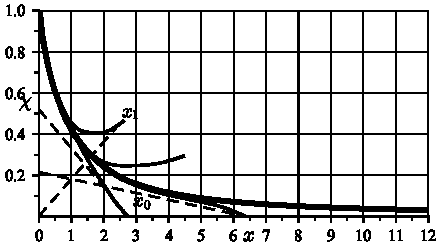
\includegraphics[width=8.5cm]{fig23.pdf}\\[0.3em]{\small 图 23}\end{minipage}\par\nopagebreak

托马斯–费米方程没有计及电子间的交换作用.这种作用的效应要比 $Z^{-2/3}$ 小一个数量级.因此，在托马斯–费米方法中计及交换作用时，还需同时计及同一数量级的其它各种效应.\footnote{这已由 А.\,С.\,Компанейц, Е.\,С.\,Павловский（ЖЭТФ 31, 927, 1956）和 Д.\,А.\,Киржниц（ЖЭТФ 32, 115, 1957）作出.}

\begin{xiti}

\noindent{\heiti 习题}\quad 试求托马斯–费米模型的中性原子中电子间静电作用能量与电子和核相互作用能量间的关系.

解：电子所产生的场势 $\varphi_e$ 可以从总势 $\varphi$ 中减去核势 $Z/r$ 而得到.因此，电子间的相互作用能量为
\begin{equation*}
\begin{aligned}[t]
  U_{ee}&=-\frac{1}{2}\int\varphi_e\,n\,\mathrm{d}V
  =\frac{Z}{2}\int\frac{n}{r}\,\mathrm{d}V-\frac{1}{2}\int\varphi\, n\,\mathrm{d}V=\\
  &=\frac{Z}{2}\int\frac{n}{r}\,\mathrm{d}V
  -\frac{(3\pi^{2})^{2/3}}{4}\int n^{5/3}\,\mathrm{d}V,
\end{aligned}
\end{equation*}
［我们已用(70.3)式以 $n$ 表达 $\varphi$］.另一方面，电子与核的相互作用能 $U_{en}$ 和它们的动能 $T$ 等于
\begin{equation*}
\begin{aligned}
  U_{en}&=-Z\int\frac{n}{r}\,\mathrm{d}V,\\
  T&=2\iint_0^{p_0}\frac{p^{2}}{2}\,4\pi p^{2}\,\mathrm{d}p\,\mathrm{d}V
  =\frac{3(3\pi^{2})^{2/3}}{10}\int n^{5/3}\,\mathrm{d}V,
\end{aligned}
\end{equation*}
把这些表式与前式比较，得关系式
\begin{equation*}
  U_{ee}=-\frac{1}{2}U_{en}-\frac{5}{6}T,
\end{equation*}
同时，按照位力定理（见《力学》§10），对按库仑定律相互作用的多粒子系统而言，我们有 $2T=-U=-U_{en}-U_{ee}$.结果得
\begin{equation*}
  U_{ee}=-\frac{1}{7}U_{en}.
\end{equation*}

\end{xiti}

\section{近核处的外电子波函数}

我们已经看到，根据托马斯–费米模型，复杂原子（$Z$ 很大）中的外电子主要处于离核 $r\sim1$ 的距离处\footnote{在这一节内，我们采用原子单位.}.但是，原子的很多性质主要取决于原子核附近的电子密度；我们将在§72和§120中考虑这些性质.为了确定这个密度的数量级，我们来追究 $r$ 从远距离（$r\sim1$）变到近距离时，原子内电子波函数 $\psi(r)$ 的变化.

在 $r\sim1$ 的区域内，核场受到其余电子的屏蔽，因而势能
\begin{equation*}
  U(r)\sim\frac{1}{r}\sim1.
\end{equation*}
这个场内电子能级的能量值 $E\sim1$.在电荷为 $Z$ 的场内，当距离具有玻尔半径的数量级 $r\sim\dfrac{1}{Z}$ 时，核场可以看成是未屏蔽的：$U=-\dfrac{Z}{r}$.在过渡区域 $1/Z\ll r\ll1$ 内，势能 $|U|$ 已比电子能量 $E$ 大很多，并且条件
\begin{equation*}
  \frac{\mathrm{d}}{\mathrm{d}r}\,\frac{1}{p}\sim\frac{\mathrm{d}}{\mathrm{d}r}\,\frac{1}{\sqrt{|U|}}\ll1
\end{equation*}
（$p$ 为动量）得以满足，因此电子的运动是准经典的.球对称的准经典波函数为
\begin{equation}
  |\psi(r)|\sim\frac{1}{r\sqrt{p}}\sim\frac{1}{r\,|U|^{1/4}},
  \quad\text{当}\ \frac{1}{Z}\ll r\ll1\ \text{时}.
\end{equation}
式中系数的数量级（$\sim1$）是由 $r\sim1$ 时 $\psi\sim1$ 的波函数“衔接”条件确定的.

$r\sim1/Z$ 时，根据(71.1)式（把 $U=-Z/r$ 代入式中）的数量级，即得近核处的波函数的值：\footnote{为了求出此式中的系数（当 $r\sim1$ 区域内的波函数为已知时），尚需利用 $r\leqslant1/Z$ 区域内的(36.25)式.}
\begin{equation}
  \psi\left(\frac{1}{Z}\right)\sim\sqrt{Z},
\end{equation}
根据有心力场内的波函数一般性质（§32），当距离进一步减小时，$\psi(r)$ 或者在数量级上保持为常数（对 s 电子），或者开始减小（当 $l\neq0$ 时）.

电子处于 $r\lesssim\dfrac{1}{Z}$ 区域内的概率为
\begin{equation}
  w\sim|\psi|^{2}r^{3}\sim\frac{1}{Z^{2}}.
\end{equation}
当然，(71.2)，(71.3)式只确定了这些量随 $Z$ 值的增大而作出的系统性变化，并没有计及从一个元素过渡到下一个元素时的非系统性变化.

\section{原子能级的精细结构}

关于电子相对论性相互作用的公式推导，属于本教程下一卷的内容（见第四卷，§33和§83）.这里只把与原子谱项有关的效应做一些一般介绍.我们发现，原子哈密顿量中的相对论项可以分成两类，其中的一类含有粒子自旋算符的线性项，另一类则包含它的二次项.前一类相当于电子轨道运动和它的自旋间的相互作用（称为自旋轨道作用）.后一类相当于电子自旋间的相互作用（自旋–自旋作用）.这两类相互作用，相对于 $v/c$ 而言（电子速度与光速之比），具有相同的数量级（二级的）；但在实际上，自旋轨道作用在重原子中远超过自旋–自旋作用.这是因为自旋轨道作用随着原子序 $Z$ 的增大而迅速增大，然而自旋间作用基本上不依赖于 $Z$（见后）.

自旋轨道作用的算符形式为
\begin{equation}
  \hat{V}_{sl}=\sum_a\hat{\boldsymbol{A}}_a\cdot\hat{\boldsymbol{s}}_a
\end{equation}
（$\sum_a$ 是对原子中的所有电子求和），式中的 $\hat{\boldsymbol{s}}_a$ 是电子自旋算符，$\hat{\boldsymbol{A}}_a$ 是某种“轨道”算符，也就是作用在坐标函数上的一个算符.在自洽场近似中，$\hat{\boldsymbol{A}}_a$ 算符与电子轨道角动量算符 $\hat{\boldsymbol{l}}_a$ 成正比，此时可把 $\hat{V}_{sl}$ 写成
\begin{equation}
  \hat{V}_{sl}=\sum\alpha_a\,\hat{\boldsymbol{l}}_a\cdot\hat{\boldsymbol{s}}_a,
\end{equation}
求和式中的系数可以通过自洽场中的电子势能 $U(r)$ 表成如下的形式：
\begin{equation}
  \alpha_a=\frac{\hbar^{2}}{2m^{2}c^{2}r_a}\,\frac{\mathrm{d}U(r_a)}{\mathrm{d}r_a}.
\end{equation}
由于 $|U(r)|$ 随 $r$ 的增大而减小，所有的 $\alpha_a>0$.

把相互作用(72.1)看作微扰时，为了计算其能量，我们必须把它对未扰态求平均.这个能量的主要贡献此时来自近核区，对电荷为 $Ze$ 的核，这个区域的距离具有玻尔半径 $\left(\sim\dfrac{\hbar^{2}}{Zme^{2}}\right)$ 的数量级.在这区域内，核场几乎不受屏蔽，因而势能为
\begin{equation*}
  U(r)\sim Z\frac{e^{2}}{r}\sim Z^{2}\frac{me^{4}}{\hbar^{2}},
\end{equation*}
于是
\begin{equation*}
  \alpha\sim\frac{\hbar^{2}U}{m^{2}c^{2}r^{2}}
  \sim Z^{4}\left(\frac{e^{2}}{\hbar c}\right)^{2}\frac{me^{4}}{\hbar^{2}},
\end{equation*}
上式乘以核附近发现电子的概率 $w$ 即得 $\alpha$ 的平均值.按照(71.3) $w\sim Z^{-2}$，因此最后求得电子的自旋轨道相互作用能为
\begin{equation*}
  \bar{\alpha}\sim\left(\frac{Ze^{2}}{\hbar c}\right)^{2}\frac{me^{4}}{\hbar^{2}},
\end{equation*}
这就是说，它和原子内的外电子的基本能量 $\left(me^{4}/\hbar^{2}\right)$ 相差一个 $(Ze^{2}/\hbar c)^{2}$ 因子.这个因子随着原子序的增长而迅速增长，对于重原子达到1的数量级.

算符(72.2)对电子未扰态的具体平均是分两步进行的.第一步，先对总角动量和总自旋的绝对值给定为 $L$ 和 $S$ 但其方向不确定的那些电子态求平均.$\hat{V}_{sl}$ 经过这样的平均以后还是一个算符，但是这个算符现在不是通过单个电子的算符表达出来，只能通过标志整个原子的算符表达出来.这些算符就是 $\hat{\boldsymbol{L}}$ 和 $\hat{\boldsymbol{S}}$.我们把经过平均以后的自旋轨道作用算符记作 $\hat{V}_{sl}$.它对 $\hat{\boldsymbol{S}}$ 呈线性，具有下列形式：
\begin{equation}
  \hat{V}_{sl}=A\,\hat{\boldsymbol{S}}\cdot\hat{\boldsymbol{L}},
\end{equation}
式中的 $A$ 是标志所给（未分裂）谱项的一个常数，亦即依赖于 $S$ 和 $L$ 但和原子总角动量 $J$ 无关的一个常数\footnote{为了弄清这个算符的含义，我们注意到，量子力学中的平均化相当于取某个合适的对角矩阵元.部分平均化相当于取一组矩阵元，这些矩阵元对描述系统状态的一部分量子数讲来是对角的.例如，在目前情形下，算符(72.2)的平均相当于构造一个矩阵，它由矩阵元 $\langle nM'_LM'_S|\,V_{sl}\,|nM_LM_S\rangle$ 所组成，其中 $M_L,M'_L$ 和 $M_S,M'_S$ 具有各种可能的数值，但对其余量子数（我们用 $n$ 代表这组量子数）则是对角的.与此相应，(72.4)中的 $\hat{\boldsymbol{S}}$ 和 $\hat{\boldsymbol{L}}$ 算符可以看作矩阵 $\langle M'_S|\,\boldsymbol{S}\,|M_S\rangle$ 和 $\langle M'_L|\,\boldsymbol{L}\,|M_L\rangle$，其矩阵元已由(27.13)式给出.在以后的某些处理中，同样需要这种分步平均化的手段.}.

为了算出简并能级（具有给定的 $S$ 和 $L$ 值）的分裂值，必须求解算符(72.4)的矩阵元所组成的久期方程.但在目前情况下，我们早已知道了使 $\hat{V}_{sl}$ 矩阵呈对角形式的正确零级近似波函数.这就是总角动量 $J$ 具有定值的状态波函数.对这样的态求平均，相当于把 $\hat{\boldsymbol{S}}\cdot\hat{\boldsymbol{L}}$ 算符换成它的本征值，根据普遍公式(31.2)，这个本征值等于
\begin{equation*}
  \boldsymbol{L}\cdot\boldsymbol{S}
  =\frac{1}{2}\left[J(J+1)-L(L+1)-S(S+1)\right].
\end{equation*}
由于 $L$ 和 $S$ 值对一个多重线的各个组分讲来都是一样的，我们所关心的又只是它们的相对位置，因此，可把多重分裂的能量写成以下形式：
\begin{equation}
  \frac{1}{2}AJ(J+1),
\end{equation}
两个相邻组分（量子数为 $J$ 和 $J-1$ 的组分）的间距因而为
\begin{equation}
  \Delta E_{J,J-1}=AJ,
\end{equation}
这个公式称为朗德间距定则（1923）.

常数 $A$ 可以是正的，也可以是负的.$A>0$ 时，多重能级的最低组分具有最小的 $J$ 值，即 $J=|L-S|$；这样的多重线称为正多重线.如果 $A<0$，多重线的最低组分则为 $J=L+S$ 的能级；这样的多重线称为倒多重线.

如果一个原子只有一个未满壳层，对这种原子的基态讲来，容易确定 $A$ 的符号.如果这个未满壳层中所装的电子数没有超过一半，则按洪德定则（§67），其中所装的 $n$ 个电子的自旋相互平行，使得总自旋具有最大可能值 $S=n/2$.把 $\boldsymbol{s}_a=\boldsymbol{S}/n$ 代入(72.2)并把 $\alpha_a$（对同一壳层内的所有电子讲来，$\alpha$ 是相同的）移到求和号外，即得
\begin{equation*}
  \hat{V}_{sl}=\frac{\alpha}{2S}\,\hat{\boldsymbol{S}}\cdot\hat{\boldsymbol{L}},
\end{equation*}
亦即 $A=\alpha/2S>0$.如果该壳层填充过半，则在(72.2)式中事先加进一个对空位（未满壳层中的空穴）求和之项，随即把它减去.由于满壳层的 $V_{sl}=0$，结果使 $\hat{V}_{sl}$ 算符具有只对空穴求和的形式
\begin{equation*}
  \hat{V}_{sl}=-\sum\alpha_a\,\hat{\boldsymbol{l}}_a\cdot\hat{\boldsymbol{s}}_a,
\end{equation*}
原子的总自旋和总轨道角动量变成 $\boldsymbol{S}=-\sum_a\hat{\boldsymbol{s}}_a$ 和 $\boldsymbol{L}=-\sum_a\hat{\boldsymbol{l}}_a$.再用以前的方法，即得 $A=-\alpha/2S$，即 $A<0$.

根据以上的分析，对于只含一个未满壳层的原子讲来，可以得出一个简单的规则，用以给出该原子的基态 $J$ 值.如果这个未满壳层中的电子数没有超过该壳层所能容纳的最大电子数的一半，则 $J=|L-S|$；如果该壳层超过了半满，则 $J=L+S$.

我们早已指出过，自旋–自旋作用不同于自旋轨道作用，它基本上不依赖于 $Z$.它是电子间的一种直接作用，显然不会包含核场.

对自旋–自旋作用算符求平均，与(72.4)式相类似，得到的表式将是 $\hat{\boldsymbol{S}}$ 的二次式.$\hat{\boldsymbol{S}}^{2}$ 和 $(\hat{\boldsymbol{S}}\cdot\hat{\boldsymbol{L}})^{2}$ 都是 $\hat{\boldsymbol{S}}$ 的二次式.前者的本征值与 $J$ 无关，不会给出谱项的分裂.因此，可把它略去，而写成
\begin{equation}
  \hat{V}_{ss}=B(\hat{\boldsymbol{S}}\cdot\hat{\boldsymbol{L}})^{2}.
\end{equation}
其中的 $B$ 是一个常数.这个算符的本征值中含有与 $J$ 无关的项，以及与 $J(J+1)$ 成正比的项，最后，还有与 $J^{2}(J+1)^{2}$ 成正比的一项.其中的第一项并不引起分裂，我们不感兴趣；第二项可以包括在(72.5)式内，只是改变了一下常数 $A$.最后，第三项给出的能量为
\begin{equation}
  \frac{1}{4}BJ^{2}(J+1)^{2}.
\end{equation}
§66—§67中讨论的原子能级构造方案，是以下列假定为基础的，即把电子的轨道角动量相加成为原子的总轨道角动量 $L$，并把它们的自旋相加成为总自旋 $S$.我们早已指出过，这种做法，只有当相对论效应很小时才是合理的；更确切地说，精细结构的间距必须远小于 $L$ 和 $S$ 值不同的那些能级之间的间距.这样的近似，称为罗素–桑德斯情形\footnote{H.~N.~Russell, F.~A.~Saunders, 1925.}，也称为“LS耦合”.

但在实际上，这种近似的适用范围是有限的.轻原子的能级是按 LS 耦合排列的，但当原子序增大时，原子中的相对论相互作用增强起来，罗素–桑德斯近似就变得不适用了\footnote{但是必须指出，尽管描述这个耦合方式的定量公式不适用了，但按这种耦合方案给出的能级分类，对较重的原子特别是对它的那些最低态（包括基态）而言，仍可能有意义.}.还应注意的是，这种近似特别不适用于高激发的能级，此时，原子中的一个电子处于 $n$ 值很大的态中，从而基本上远离原子核（§68）.这个电子和其它运动电子间的静电作用比较弱；可是，“原子实”中的相对论相互作用并不因此减小.

在相反的极端情形下，相对论作用远超过静电作用（更精确地说，远超过依赖于 $L$ 和 $S$ 的那部分能量）.这个时候，我们不能把轨道角动量和自旋分开来处理，因为它们不再守恒.每个单电子用它的总角动量 $j$ 来标志，由 $j$ 相加成为原子的总角动量 $J$.原子能级的这种构造方式称为“$jj$ 耦合”.实际上，我们并没有在纯态中碰到过 $jj$ 耦合，但是介于 LS 和 $jj$ 耦合之间的各种耦合方式，曾在极重原子的能级中观测到\footnote{关于各种耦合方案及其定量方面的问题，详见下书：E.~U.~Condon, G.~H.~Shortley；The Theory of Atomic Spectra, Cambridge University Press, 1935.}.

还有一种独特的耦合方式，曾在某些高激发态中观测到.此时的“原子实”仍可处于罗素–桑德斯态中，也就是以 $L$ 和 $S$ 值为标志的态中，但是它与高激发电子间的耦合则是 $jj$ 型的；其原因仍是由于这个电子的静电作用比较弱.

氢原子能级的精细结构具有某些特殊性.它将在本教程的第四卷中作出精确计算（第四卷，§34）.这里只须指出，当主量子数 $n$ 给定后，能量只与电子的总角动量 $j$ 有关.因此，它的能级简并度并没有完全消除掉；对一个具有给定 $n$ 和 $j$ 值的能级讲来，就有轨道角动量为 $l=j\pm1/2$ 的两个态（除非 $j$ 值等于 $n-\dfrac{1}{2}$，这是 $n$ 给定后的最大 $j$ 值）.例如，$n=3$ 的能级分裂成为三个能级，其中的 $s_{\frac{1}{2}}$，$p_{\frac{1}{2}}$ 态属于一个能级，$p_{\frac{3}{2}}$ 和 $d_{\frac{3}{2}}$ 态属于另一个能级，$d_{\frac{5}{2}}$ 则属于第三个能级.

\section{门捷列夫元素周期系}

元素按原子序的递增次序排列以后，呈现出性质上的周期性变化\footnote{Д.\,И.\,Менделеев, 1869.}，要阐明这种变化的本质，必须研究原子的各个电子壳层逐步被填充时的特点.周期系的理论是由玻尔\footnote{N.~Bohr, 1922.}提出的.

从一个原子过渡到下一个原子时，电荷增加1，并有一个电子添入壳层中.初想起来，每个相继添入的电子，它的结合能似应随原子序的增大而单调地递增.但实际变化却完全不是这样.

基态氢原子中，只有一个处于 1s 态的电子.下一个元素氦的原子中，添加了另一个 1s 电子，可是氦原子内每个 1s 电子的结合能要比氢原子内的电子结合能大很多.这是一种自然的结果，因为氢原子内电子所处的电场不同于添加到 $\mathrm{He}^{+}$ 离子内的一个电子所处的电场.这两个电场在远距处近似地相同，但在近核处，$Z=2$ 的 $\mathrm{He}^{+}$ 离子的电场则比 $Z=1$ 的氢核场强得多.在锂原子（$Z=3$）中，第三个电子只能填入 2s 态，因为 1s 态中不可能同时存在比两个多的电子.对一个给定的 $Z$ 值而言，2s 能级高于 1s 能级；但这两个能级都随核电荷的增加而下降.但从 $Z=2$ 过渡到 $Z=3$ 时，前一种效应是主要的，所以 Li 原子中第三个电子的结合能远小于氦原子中电子的结合能.再往下，从 $\mathrm{Be}\ (Z=4)$ 原子到 $\mathrm{Ne}\ (Z=10)$ 原子，先填入一个 2s 电子，再陆续填入 6 个 2p 电子.这些电子的结合能，由于核电荷的增大而平均地增大.再下一个电子的添入，轮到 $\mathrm{Na}\ (Z=11)$ 原子，它只能填到 3s 态，由于这个填入更高壳层内的效应要大于核电荷增大的效应，所以结合能再次显著地下降.

电子壳层的上述填充图像反映了各元素构成的整个系列的特征.全部电子态可以分成若干个依次被填充的组，当每组中的各态依次被填充时，结合能平均地增大，但当轮到下一组的态开始被填充时，结合能又显著地下降.

图24是用光谱学数据绘出的元素电离势；这些电离势确定了一个元素过渡到下一个元素时所填入电子的结合能.

\par\nopagebreak\noindent\begin{minipage}{\linewidth}\centering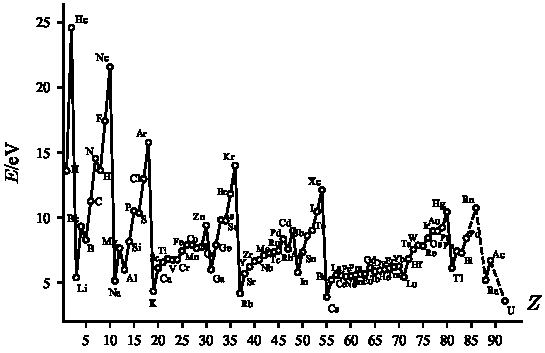
\includegraphics[width=10cm]{fig24.pdf}\\[0.3em]{\small 图 24}\end{minipage}\par\nopagebreak

各种不同的态按下列方式分成若干个依次被填充的组：
\begin{equation}
\left.\begin{array}{llr}
1s & \cdots\cdots\cdots\cdots\cdots & \text{2 个电子}\\
2s,2p & \cdots\cdots\cdots\cdots\cdots & \text{8 个电子}\\
3s,3p & \cdots\cdots\cdots\cdots\cdots & \text{8 个电子}\\
4s,3d,4p & \cdots\cdots\cdots\cdots & \text{18 个电子}\\
5s,4d,5p & \cdots\cdots\cdots\cdots & \text{18 个电子}\\
6s,4f,5d,6p & \cdots\cdots\cdots & \text{32 个电子}\\
7s,6d,5f & \cdots\cdots\cdots\cdots &
\end{array}\right\}
\end{equation}
第一组被 H 和 He 填充完毕；第二组和第三组的填充相当于周期表中的前两个（短）周期，每个周期含有8个元素.随后是两个长周期，每个周期含有18个元素，还有一个包括稀土元素在内的长周期，共含32个元素.最后一组的态对自然界的现有元素（以及人造的超铀元素）讲来还未被填满.

为了理解每组的态被陆续填充时元素性质上的变化，指出 d 和 f 态不同于 s 和 p 态的下列特性是十分重要的.对重原子内的一个电子讲来，有心力场（由静电场及离心场相加而成）的有效势能曲线，在原点附近有一个急剧的近乎垂直的下降，降到某一很深的极小值后，再回升起来，然后渐近地趋于零.对于 s 态和 p 态，这些曲线的上升部分彼此靠得很近.这就表明，这些态中的电子与原子核的距离差不多相等.反之，d 态特别是 f 态的曲线要向左移得很多；这些曲线所确定的“经典通区”，比具有同一电子总能量的各 s 态和 p 态更为靠近原子核.换句话说，d 态和 f 态的电子，大体上要比 s 态和 p 态的电子更加靠近原子核.

原子的许多性质（包括元素的化学性质，见§81）主要取决于电子壳层的外壳层.从这一点讲来，d 态和 f 态的上述特点是非常重要的.例如，当 4f 态开始填充时（见下面的稀土元素），新添入的电子要比先填入的电子更加靠近原子核，结果，使这些新添电子对元素的化学性质差不多不发生影响，所有的稀土元素就有十分相似的化学性质.

含有闭合 d 壳层和闭合 f 壳层（或者完全不含这些壳层）的元素，称为主族元素；d 和 f 态正在填充中的元素称为过渡族元素.我们最好把这两族元素分开来考虑.

先考虑主族元素.氢和氦具有下列基态
\begin{equation*}
  {}_{1}\mathrm{H}:1\mathrm{s}^{2}\,{}^{2}\mathrm{S}_{1/2},
  \qquad
  {}_{2}\mathrm{He}:1\mathrm{s}^{2}\,{}^{1}\mathrm{S}_{0}
\end{equation*}
（化学符号左下角的数字代表原子序）.其余主族元素的电子组态见表3.

\begin{center}
{\heiti 表 3}\quad 主族元素中原子的电子组态\\[0.8em]
\small\setlength{\tabcolsep}{3.2pt}%
\begin{tabular}{|c||c|c|c|c|c|c|c|c||c|}
\hline
 & $\mathrm{s}$ & $\mathrm{s}^{2}$ & $\mathrm{s}^{2}\mathrm{p}$ & $\mathrm{s}^{2}\mathrm{p}^{2}$ & $\mathrm{s}^{2}\mathrm{p}^{3}$ & $\mathrm{s}^{2}\mathrm{p}^{4}$ & $\mathrm{s}^{2}\mathrm{p}^{5}$ & $\mathrm{s}^{2}\mathrm{p}^{6}$ & \\
\hline
$n=2$ & ${}_{3}\mathrm{Li}$ & ${}_{4}\mathrm{Be}$ & ${}_{5}\mathrm{B}$ & ${}_{6}\mathrm{C}$ & ${}_{7}\mathrm{N}$ & ${}_{8}\mathrm{O}$ & ${}_{9}\mathrm{F}$ & ${}_{10}\mathrm{Ne}$ & $1\mathrm{s}^{2}$\\
3 & ${}_{11}\mathrm{Na}$ & ${}_{12}\mathrm{Mg}$ & ${}_{13}\mathrm{Al}$ & ${}_{14}\mathrm{Si}$ & ${}_{15}\mathrm{P}$ & ${}_{16}\mathrm{S}$ & ${}_{17}\mathrm{Cl}$ & ${}_{18}\mathrm{Ar}$ & $2\mathrm{s}^{2}2\mathrm{p}^{6}$\\
4 & ${}_{19}\mathrm{K}$ & ${}_{20}\mathrm{Ca}$ & & & & & & & $3\mathrm{s}^{2}3\mathrm{p}^{6}$\\
4 & ${}_{29}\mathrm{Cu}$ & ${}_{30}\mathrm{Zn}$ & ${}_{31}\mathrm{Ga}$ & ${}_{32}\mathrm{Ge}$ & ${}_{33}\mathrm{As}$ & ${}_{34}\mathrm{Se}$ & ${}_{35}\mathrm{Br}$ & ${}_{36}\mathrm{Kr}$ & $3\mathrm{d}^{10}$\\
5 & ${}_{37}\mathrm{Rb}$ & ${}_{38}\mathrm{Sr}$ & & & & & & & $4\mathrm{s}^{2}4\mathrm{p}^{6}$\\
5 & ${}_{47}\mathrm{Ag}$ & ${}_{48}\mathrm{Cd}$ & ${}_{49}\mathrm{In}$ & ${}_{50}\mathrm{Sn}$ & ${}_{51}\mathrm{Sb}$ & ${}_{52}\mathrm{Te}$ & ${}_{53}\mathrm{I}$ & ${}_{54}\mathrm{Xe}$ & $4\mathrm{d}^{10}$\\
6 & ${}_{55}\mathrm{Cs}$ & ${}_{56}\mathrm{Ba}$ & & & & & & & $5\mathrm{s}^{2}5\mathrm{p}^{6}$\\
6 & ${}_{79}\mathrm{Au}$ & ${}_{80}\mathrm{Hg}$ & ${}_{81}\mathrm{Tl}$ & ${}_{82}\mathrm{Pb}$ & ${}_{83}\mathrm{Bi}$ & ${}_{84}\mathrm{Po}$ & ${}_{85}\mathrm{At}$ & ${}_{86}\mathrm{Rn}$ & $4\mathrm{f}^{14}5\mathrm{d}^{10}$\\
7 & ${}_{87}\mathrm{Fr}$ & ${}_{88}\mathrm{Ra}$ & & & & & & & $6\mathrm{s}^{2}6\mathrm{p}^{6}$\\
\hline
 & ${}^{2}\mathrm{S}_{1/2}$ & ${}^{1}\mathrm{S}_{0}$ & ${}^{2}\mathrm{P}_{1/2}$ & ${}^{3}\mathrm{P}_{0}$ & ${}^{4}\mathrm{S}_{3/2}$ & ${}^{3}\mathrm{P}_{2}$ & ${}^{2}\mathrm{P}_{3/2}$ & ${}^{1}\mathrm{S}_{0}$ & \\
\hline
\end{tabular}
\end{center}

\emergencystretch=3em%
每个原子的闭合壳层见表中该行及以上各行的右端.它的未满壳层的电子组态见同列之首，这些态中电子的主量子数见同行的左端.整个原子的基态见表底.例如，铝原子的电子组态为 $1\mathrm{s}^{2}2\mathrm{s}^{2}2\mathrm{p}^{6}\allowbreak 3\mathrm{s}^{2}3\mathrm{p}^{2}\,{}^{2}\mathrm{P}_{1/2}$.
\emergencystretch=0pt%

基态原子的 $L$ 和 $S$ 值可按洪德定则（§67）确定（电子的组态为已知），$J$ 值则按§72中指出的规则确定.

惰性气体的原子（He, Ne, Ar, Kr, Xe, Rn）在表中占有特殊的地位：每个原子正好是把(73.1)中列举的一个组态完全填满.它们的电子组态具有异常的稳定性（它们的电离势在其所属的系内都是最大的）.这就产生了这些元素的化学惰性.

我们看到，主族元素中不同态的填充次序是极有规则的：对每一个主量子数 $n$ 而言，总是先填 s 态再填 p 态.这些元素的离子的电子组态也是很有规则的（直到把 d 或 f 壳层中的电子电离掉为止）：每个离子具有和前一个原子相应的组态.例如，$\mathrm{Mg}^{+}$ 离子具有 Na 原子的组态，$\mathrm{Mg}^{++}$ 离子具有 Ne 原子的组态.

现在来考虑过渡族元素.3d, 4d, 5d 壳层正在填充中的元素分别称为铁族，钯族和铂族元素.表4中列出了这几族元素的电子组态及原子谱项，它们是从光谱学数据得知的.由表4可知，d 壳层的填充要比主族元素中 s 和 p 壳层的填充不规则得很多.表中有一个主要特征是 s 态和 d 态间的“竞争”现象.这表现于下列事实，当 $p$ 增加时，往往不按正规次序填成 $\mathrm{d}^{p}\mathrm{s}^{2}$ 组态，而出现 $\mathrm{d}^{p+1}\mathrm{s}$ 型或 $\mathrm{d}^{p+2}$ 型的组态.例如，铁族元素中，Cr 原子的组态是 $3\mathrm{d}^{5}4\mathrm{s}$ 而不是 $3\mathrm{d}^{4}4\mathrm{s}^{2}$；在含有8个 d 电子的 Ni 之后，立刻是 d 壳层被完全填满的 Cu 原子（铜原子因此放在主族中）.这样的不规则性也能在离子的谱项中观察到：这些离子的电子组态，一般讲来，与前一个原子的组态并不完全一致.例如，$\mathrm{V}^{+}$ 离子具有 $3\mathrm{d}^{4}$ 的组态（不是 Ti 原子的 $3\mathrm{d}^{2}4\mathrm{s}^{2}$ 组态）；$\mathrm{Fe}^{+}$ 离子具有 $3\mathrm{d}^{6}4\mathrm{s}$ 的组态（不是 Mn 原子的 $3\mathrm{d}^{5}4\mathrm{s}^{2}$ 组态）.我们可以指出，在晶体及溶液中所有自然状态的离子，它们的未满壳层中只含 d 电子（不含 s 或 p 电子）.例如，晶体或溶液中找到的铁离子只有 $\mathrm{Fe}^{++}$ 和 $\mathrm{Fe}^{+++}$，它们的组态分别为 $3\mathrm{d}^{6}$ 和 $3\mathrm{d}^{5}$.

\begin{center}
{\heiti 表 4}\quad 铁族，钯族和铂族元素中原子的电子组态

\vspace{0.6em}
铁\quad 族\\[0.5em]
\small\setlength{\tabcolsep}{2.5pt}%
\begin{tabular}{|c||c|c|c|c|c|c|c|c|}
\hline
Ar 壳层+ & ${}_{21}\mathrm{Sc}$ & ${}_{22}\mathrm{Ti}$ & ${}_{23}\mathrm{V}$ & ${}_{24}\mathrm{Cr}$ & ${}_{25}\mathrm{Mn}$ & ${}_{26}\mathrm{Fe}$ & ${}_{27}\mathrm{Co}$ & ${}_{28}\mathrm{Ni}$\\
\hline
 & $\begin{array}{c}3\mathrm{d}4\mathrm{s}^{2}\\{}^{2}\mathrm{D}_{3/2}\end{array}$ &
$\begin{array}{c}3\mathrm{d}^{2}4\mathrm{s}^{2}\\{}^{3}\mathrm{F}_{2}\end{array}$ &
$\begin{array}{c}3\mathrm{d}^{3}4\mathrm{s}^{2}\\{}^{4}\mathrm{F}_{3/2}\end{array}$ &
$\begin{array}{c}3\mathrm{d}^{5}4\mathrm{s}\\{}^{7}\mathrm{S}_{3}\end{array}$ &
$\begin{array}{c}3\mathrm{d}^{5}4\mathrm{s}^{2}\\{}^{6}\mathrm{S}_{5/2}\end{array}$ &
$\begin{array}{c}3\mathrm{d}^{6}4\mathrm{s}^{2}\\{}^{5}\mathrm{D}_{4}\end{array}$ &
$\begin{array}{c}3\mathrm{d}^{7}4\mathrm{s}^{2}\\{}^{4}\mathrm{F}_{9/2}\end{array}$ &
$\begin{array}{c}3\mathrm{d}^{8}4\mathrm{s}^{2}\\{}^{3}\mathrm{F}_{4}\end{array}$\\
\hline
\end{tabular}

\vspace{0.8em}
钯\quad 族\\[0.5em]
\begin{tabular}{|c||c|c|c|c|c|c|c|c|}
\hline
Kr 壳层+ & ${}_{39}\mathrm{Y}$ & ${}_{40}\mathrm{Zr}$ & ${}_{41}\mathrm{Nb}$ & ${}_{42}\mathrm{Mo}$ & ${}_{43}\mathrm{Tc}$ & ${}_{44}\mathrm{Ru}$ & ${}_{45}\mathrm{Rh}$ & ${}_{46}\mathrm{Pd}$\\
\hline
 & $\begin{array}{c}4\mathrm{d}5\mathrm{s}^{2}\\{}^{2}\mathrm{D}_{3/2}\end{array}$ &
$\begin{array}{c}4\mathrm{d}^{2}5\mathrm{s}^{2}\\{}^{3}\mathrm{F}_{2}\end{array}$ &
$\begin{array}{c}4\mathrm{d}^{4}5\mathrm{s}\\{}^{6}\mathrm{D}_{1/2}\end{array}$ &
$\begin{array}{c}4\mathrm{d}^{5}5\mathrm{s}\\{}^{7}\mathrm{S}_{3}\end{array}$ &
$\begin{array}{c}4\mathrm{d}^{5}5\mathrm{s}^{2}\\{}^{6}\mathrm{S}_{5/2}\end{array}$ &
$\begin{array}{c}4\mathrm{d}^{7}5\mathrm{s}\\{}^{5}\mathrm{F}_{5}\end{array}$ &
$\begin{array}{c}4\mathrm{d}^{8}5\mathrm{s}\\{}^{4}\mathrm{F}_{9/2}\end{array}$ &
$\begin{array}{c}4\mathrm{d}^{10}\\{}^{1}\mathrm{S}_{0}\end{array}$\\
\hline
\end{tabular}

\vspace{0.8em}
铂\quad 族\\[0.5em]
\begin{tabular}{|c||c|c|c|c|c|c|c|c|}
\hline
Xe 壳层+ & ${}_{57}\mathrm{La}$ & & & & & & & \\
\hline
 & $\begin{array}{c}5\mathrm{d}6\mathrm{s}^{2}\\{}^{2}\mathrm{D}_{3/2}\end{array}$ & & & & & & & \\
\hline
Xe 壳层$+4\mathrm{f}^{14}+$ & ${}_{71}\mathrm{Lu}$ & ${}_{72}\mathrm{Hf}$ & ${}_{73}\mathrm{Ta}$ & ${}_{74}\mathrm{W}$ & ${}_{75}\mathrm{Re}$ & ${}_{76}\mathrm{Os}$ & ${}_{77}\mathrm{Ir}$ & ${}_{78}\mathrm{Pt}$\\
\hline
 & $\begin{array}{c}5\mathrm{d}6\mathrm{s}^{2}\\{}^{2}\mathrm{D}_{3/2}\end{array}$ &
$\begin{array}{c}5\mathrm{d}^{2}6\mathrm{s}^{2}\\{}^{3}\mathrm{F}_{2}\end{array}$ &
$\begin{array}{c}5\mathrm{d}^{3}6\mathrm{s}^{2}\\{}^{4}\mathrm{F}_{3/2}\end{array}$ &
$\begin{array}{c}5\mathrm{d}^{4}6\mathrm{s}^{2}\\{}^{5}\mathrm{D}_{0}\end{array}$ &
$\begin{array}{c}5\mathrm{d}^{5}6\mathrm{s}^{2}\\{}^{6}\mathrm{S}_{5/2}\end{array}$ &
$\begin{array}{c}5\mathrm{d}^{6}6\mathrm{s}^{2}\\{}^{5}\mathrm{D}_{4}\end{array}$ &
$\begin{array}{c}5\mathrm{d}^{7}6\mathrm{s}^{2}\\{}^{4}\mathrm{F}_{9/2}\end{array}$ &
$\begin{array}{c}5\mathrm{d}^{9}6\mathrm{s}\\{}^{3}\mathrm{D}_{3}\end{array}$\\
\hline
\end{tabular}
\end{center}

类似的情况也出现在 4f 壳层的填充中，这些元素称为稀土族元素（表5）\footnote{有些化学书上往往把 Lu 也算在稀土元素内.但这是不正确的，由于 Lu 中的 4f 壳层已被填满；因此必须按表 4 所示放在铂族内.}.4f 壳层的填充也是不太规则的，其特点是 4f, 5d 和 6s 态间的“竞争”.

\begin{center}
{\heiti 表 5}\quad 稀土族元素中原子的电子组态\\[0.8em]
\small\setlength{\tabcolsep}{2.5pt}%
\begin{tabular}{|c||c|c|c|c|c|c|c|}
\hline
Xe 壳层+ & ${}_{58}\mathrm{Ce}$ & ${}_{59}\mathrm{Pr}$ & ${}_{60}\mathrm{Nd}$ & ${}_{61}\mathrm{Pm}$ & ${}_{62}\mathrm{Sm}$ & ${}_{63}\mathrm{Eu}$ & \\
\hline
 & $\begin{array}{c}4\mathrm{f}5\mathrm{d}6\mathrm{s}^{2}\\{}^{1}\mathrm{G}_{4}\end{array}$ &
$\begin{array}{c}4\mathrm{f}^{3}6\mathrm{s}^{2}\\{}^{4}\mathrm{I}_{9/2}\end{array}$ &
$\begin{array}{c}4\mathrm{f}^{4}6\mathrm{s}^{2}\\{}^{5}\mathrm{I}_{4}\end{array}$ &
$\begin{array}{c}4\mathrm{f}^{5}6\mathrm{s}^{2}\\{}^{6}\mathrm{H}_{5/2}\end{array}$ &
$\begin{array}{c}4\mathrm{f}^{6}6\mathrm{s}^{2}\\{}^{7}\mathrm{F}_{0}\end{array}$ &
$\begin{array}{c}4\mathrm{f}^{7}6\mathrm{s}^{2}\\{}^{8}\mathrm{S}_{7/2}\end{array}$ & \\
\hline
 & ${}_{64}\mathrm{Gd}$ & ${}_{65}\mathrm{Tb}$ & ${}_{66}\mathrm{Dy}$ & ${}_{67}\mathrm{Ho}$ & ${}_{68}\mathrm{Er}$ & ${}_{69}\mathrm{Tm}$ & ${}_{70}\mathrm{Yb}$\\
\hline
 & $\begin{array}{c}4\mathrm{f}^{7}5\mathrm{d}6\mathrm{s}^{2}\\{}^{9}\mathrm{D}_{2}\end{array}$ &
$\begin{array}{c}4\mathrm{f}^{8}6\mathrm{s}^{2}\\{}^{6}\mathrm{H}_{15/2}\end{array}$ &
$\begin{array}{c}4\mathrm{f}^{10}6\mathrm{s}^{2}\\{}^{5}\mathrm{I}_{8}\end{array}$ &
$\begin{array}{c}4\mathrm{f}^{11}6\mathrm{s}^{2}\\{}^{4}\mathrm{I}_{15/2}\end{array}$ &
$\begin{array}{c}4\mathrm{f}^{12}6\mathrm{s}^{2}\\{}^{3}\mathrm{H}_{6}\end{array}$ &
$\begin{array}{c}4\mathrm{f}^{13}6\mathrm{s}^{2}\\{}^{2}\mathrm{F}_{7/2}\end{array}$ &
$\begin{array}{c}4\mathrm{f}^{14}6\mathrm{s}^{2}\\{}^{1}\mathrm{S}_{0}\end{array}$\\
\hline
\end{tabular}
\end{center}

最后一族过渡元素是从锕开始的.与稀土族元素相类似，锕族元素填充着 6d 和 5f 壳层（表6\mbox{）.}

\begin{center}
{\heiti 表 6}\quad 锕族元素中原子的电子组态\\[0.8em]
\small\setlength{\tabcolsep}{2.5pt}%
\begin{tabular}{|c||c|c|c|c|c|c|c|c|}
\hline
Rn 壳层+ & ${}_{89}\mathrm{Ac}$ & ${}_{90}\mathrm{Th}$ & ${}_{91}\mathrm{Pa}$ & ${}_{92}\mathrm{U}$ & ${}_{93}\mathrm{Np}$ & ${}_{94}\mathrm{Pu}$ & ${}_{95}\mathrm{Am}$ & ${}_{96}\mathrm{Cm}$\\
\hline
 & $\begin{array}{c}6\mathrm{d}7\mathrm{s}^{2}\\{}^{2}\mathrm{D}_{3/2}\end{array}$ &
$\begin{array}{c}6\mathrm{d}^{2}7\mathrm{s}^{2}\\{}^{3}\mathrm{F}_{2}\end{array}$ &
$\begin{array}{c}5\mathrm{f}^{2}6\mathrm{d}7\mathrm{s}^{2}\\{}^{4}\mathrm{K}_{11/2}\end{array}$ &
$\begin{array}{c}5\mathrm{f}^{3}6\mathrm{d}7\mathrm{s}^{2}\\{}^{5}\mathrm{L}_{6}\end{array}$ &
$\begin{array}{c}5\mathrm{f}^{4}6\mathrm{d}7\mathrm{s}^{2}\\{}^{6}\mathrm{L}_{11/2}\end{array}$ &
$\begin{array}{c}5\mathrm{f}^{6}7\mathrm{s}^{2}\\{}^{7}\mathrm{F}_{0}\end{array}$ &
$\begin{array}{c}5\mathrm{f}^{7}7\mathrm{s}^{2}\\{}^{8}\mathrm{S}_{7/2}\end{array}$ &
$\begin{array}{c}5\mathrm{f}^{7}6\mathrm{d}7\mathrm{s}^{2}\\{}^{9}\mathrm{D}_{2}\end{array}$\\
\hline
\end{tabular}
\end{center}

作为本节的结束，我们来讨论一下托马斯–费米方法的一个有趣应用.我们看到，p 壳层中的电子首先出现在第五号元素 B（硼）中，d 电子首先出现在 $Z=21$ 的 Sc（钪）中，f 电子首先出现在 $Z=58$ 的 Ce（铈）中.这些 $Z$ 值可用托马斯–费米方法预言出来，其法如下.

复杂原子内轨道角动量为 $l$ 的电子是以下列有效势能运动的\footnote{和 §70 一样，我们采用原子单位.}：
\begin{equation*}
  U_l(r)=-\varphi(r)+\frac{\left(l+\dfrac{1}{2}\right)^{2}}{2r^{2}}.
\end{equation*}
第一项是托马斯–费米势 $\varphi(r)$ 所描述的电场中的势能.第二项是离心能，因为运动是准经典的，所以其中的 $l(l+1)$ 已改为 $\left(l+\dfrac{1}{2}\right)^{2}$.由于原子中的电子总能量是负的，如果 $U_l(r)$ 对所有的 $r$ 讲来都有 $U_l(r)>0$（$Z$ 和 $l$ 为给定），那么该原子中显然不可能存在具有所给 $l$ 值的电子.如果固定 $l$ 值而变 $Z$，我们发现，当 $Z$ 值足够小时，实际上到处都有 $U_l(r)>0$.当 $Z$ 值增大达到某一值时，$U_l=U_l(r)$ 曲线开始和横轴相接触；$Z$ 值再大时，就会出现 $U_l(r)<0$ 的区域.因此具有给定 $l$ 值的电子首次在原子中出现时所需的 $Z$ 值，是由 $U_l(r)$ 曲线与横轴相切的条件确定的，也就是由以下两式确定的：
\begin{equation*}
  U_l(r)=-\varphi+\frac{\left(l+\dfrac{1}{2}\right)^{2}}{2r^{2}}=0,
\end{equation*}
\begin{equation*}
  U'_l(r)=-\varphi'(r)-\frac{\left(l+\dfrac{1}{2}\right)^{2}}{r^{3}}=0.
\end{equation*}
把(70.6)式的势代入上式，得下列方程：
\begin{equation}
\left.\begin{aligned}
  &Z^{2/3}\frac{\chi(x)}{x}
  =\left(\frac{4}{3\pi}\right)^{2/3}
  \frac{\left(l+\dfrac{1}{2}\right)^{2}}{x^{2}},\\
  &Z^{2/3}\frac{x\chi'(x)-\chi(x)}{x}
  =-2\left(\frac{4}{3\pi}\right)^{2/3}
  \frac{\left(l+\dfrac{1}{2}\right)^{2}}{x^{2}}.
\end{aligned}\right\}
\end{equation}
第一式的两边除以第二式的两边，即得 $x$ 的方程式
\begin{equation*}
  \frac{\chi'(x)}{\chi(x)}=-\frac{1}{x},
\end{equation*}
然后，用(73.2)的第一式求 $Z$.数值计算后，得
\begin{equation*}
  Z=0.155(2l+1)^{3},
\end{equation*}
这个式子表出了具有给定 $l$ 值的电子首次在原子中出现时的 $Z$ 值；其误差约 $10\%$.如果把系数 0.155 改成 0.17，可得很精确的结果：
\begin{equation}
  Z=0.17(2l+1)^{3},
\end{equation}
$l=1,2,3$ 时，上式四舍五入取最近整数值后，即得正确值 5, 21, 58.$l=4$ 时，(73.3)式给出 $Z=124$；这表明 g 电子要在第124号元素中才能首次出现.

\section{X 射线谱项}

原子中内电子的结合能如此之大，以致当这样一个内电子跃迁到未满的外壳层中（或脱离原子）时，这个受激原子（或离子）相对于电离来讲将处于力学上的不稳定状态，伴随着这种电离，将发生电子壳层的重建并形成稳定的离子.但由于原子中电子间的相互作用比较弱，产生这种跃迁的概率比较小，因而激发态的寿命 $\tau$ 比较长.由于能级“宽度” $\hbar/\tau$ 比较小（见§44），我们就有理由把具有受激内电子的原子能量，看作该原子的一些“准定态”离散能级.这些能级称为 X 射线谱项\footnote{这个名称的来源，是由于这些能级间的跃迁引起该原子发射出 X 射线.}.

X 射线谱项的分类，主要根据移去电子的那个封闭壳层，也就是形成“空穴”的那个电子壳层而定.至于这个电子究竟移到了哪一个外壳层，这对原子的能量几乎没有什么影响，因而是不重要的.

填满某一壳层的一组电子，它们的总角动量等于零.去掉一个电子以后，这个壳层获得某一角动量 $j$.对 $(n,l)$ 壳层讲来，角动量 $j$ 显然可取 $l\pm\dfrac{1}{2}$ 两个值.因此，所得的能级可以记作 $1\mathrm{s}_{1/2}$，$2\mathrm{s}_{1/2}$，$2\mathrm{p}_{1/2}$，$2\mathrm{p}_{3/2}$，$\cdots$，其中的 $j$ 值是作为下标附记在指示空穴所在的字母下的.但在习惯上，常用以下的专门记号代表这些能级：
\begin{equation*}
\begin{array}{ccccccccc}
1\mathrm{s}_{1/2}, & 2\mathrm{s}_{1/2}, & 2\mathrm{p}_{1/2}, & 2\mathrm{p}_{3/2}, &
3\mathrm{s}_{1/2}, & 3\mathrm{p}_{1/2}, & 3\mathrm{p}_{3/2}, &
3\mathrm{d}_{3/2}, & 3\mathrm{d}_{5/2},\cdots\\
\mathrm{K} & \mathrm{L}_{\mathrm{I}} & \mathrm{L}_{\mathrm{II}} & \mathrm{L}_{\mathrm{III}} &
\mathrm{M}_{\mathrm{I}} & \mathrm{M}_{\mathrm{II}} & \mathrm{M}_{\mathrm{III}} &
\mathrm{M}_{\mathrm{IV}} & \mathrm{M}_{\mathrm{V}}\cdots
\end{array}
\end{equation*}
$n=4,5,6$ 的能级相应地用 N, O, P 等字母标记之.

$n$ 值相同的那些能级彼此靠得很近（用同一大写字母标记之），而与不同 $n$ 值的那些能级远离.其原因在于这些内电子离核相对来说较近，电子所处的场差不多是未屏蔽的核场.与此相应，它们的态是“类氢”态，它们的能量在一级近似中等于 $-Z^{2}/2n^{2}$（用原子单位），也就是只和 $n$ 有关.考虑了相对论效应以后，$j$ 值不同的谱项就彼此分开（参阅§72关于氢原子能级精细结构的讨论），例如，$\mathrm{L}_{\mathrm{I}}$，$\mathrm{L}_{\mathrm{II}}$ 与 $\mathrm{L}_{\mathrm{III}}$ 分开；$\mathrm{M}_{\mathrm{I}}$，$\mathrm{M}_{\mathrm{II}}$ 与 $\mathrm{M}_{\mathrm{III}}$，$\mathrm{M}_{\mathrm{IV}}$ 分开.这样的一对能级称为相对论双线.$j$ 值相同 $l$ 值不同的谱项（例如 $\mathrm{L}_{\mathrm{I}}$ 和 $\mathrm{L}_{\mathrm{II}}$，$\mathrm{M}_{\mathrm{I}}$ 和 $\mathrm{M}_{\mathrm{II}}$），它们的分裂是由于内电子所处的场已与核库仑场有所不同，也就是这时计及了该电子与其它电子的相互作用.这样的一对能级称为屏蔽双线.其余电子在核附近产生的势是电子“类氢”能量的主要修正项，它与 $Z^{4/3}$ 成正比［见(70.8)］.但由于这个修正项既和 $n$ 无关，也和 $l$ 无关，它并不影响到能级间距.因此，能级差的主要修正项来自一个电子与其邻近电子间的相互作用.由于内电子间的间距 $r\sim1/Z$（在电荷为 $Z$ 的场内的玻尔半径），上述作用的能量为 $\sim1/r\sim Z$.考虑了这个修正后，在同样的精度内，可以把 X 射线谱项的能量写作 $-(Z-\delta)^{2}/2n^{2}$，其中的 $\delta=\delta(n,l)$ 是一个比 $Z$ 小很多的量，可看作核电荷的屏蔽值.

除了电子壳层内一个“空穴”的 X 射线谱项外，也可能存在两个和三个“空穴”的谱项.由于内电子的自旋轨道作用很强，故空穴的相互耦合为 $jj$ 耦合.

X 射线谱项的宽度取决于重建电子壳层从而填充该空穴的各种可能过程的总概率.在重原子中，最重要的过程是空穴从所给壳层跃迁到更高壳层（也就是电子相反的跃迁），从而辐射出 X 射线光量子的过程.这种“辐射”跃迁的概率（及其所对应的那部分能级宽度）随着原子序的增大而极快地增长（约正比于 $Z^{4}$），但对给定的 $Z$ 则随跃迁能级的增高而减小.

对于较轻原子（和较高能级），无辐射跃迁占有重要的甚至优势的地位，此时空穴被更高能量的电子所填补，它所释放的能量，可以把原子中的另一个内电子剥离出去（称为俄歇效应），此过程的结果，使该原子处于具有两个空穴的态中.这个过程的概率及其所贡献的那部分能级宽度，在一级近似（相对于 $1/Z$）下与原子序无关\footnote{举例来说，K 能级的俄歇宽度约为 1 eV，更高能级的俄歇宽度可达 $\sim$10 eV.}（参阅例题）.

\begin{xiti}

\noindent{\heiti 习题}\quad 当原子序足够大时，求 X 射线谱项的俄歇宽度依赖于原子序的极限定律.

解：俄歇跃迁概率与下列矩阵元的平方成正比：
\begin{equation*}
  M=\iint\psi_1'^{\,*}\psi_2'^{\,*}\,V\psi_1\psi_2\,\mathrm{d}V_1\mathrm{d}V_2,
\end{equation*}
其中的 $\psi_1\psi_2$ 和 $\psi'_1\psi'_2$ 是参与跃迁过程的那两个电子的初末态波函数，而 $V=e^{2}/r_{12}$ 是它们的相互作用能量.当 $Z$ 足够大时，内电子的波函数可看成类氢波函数，并可略去其余电子对核场的屏蔽（在原子内部对积分式 $M$ 有贡献的那个区域内，电离电子的波函数也是类氢的）.如果把所有的量表成库仑单位（常数 $\alpha=Ze^{2}$，见§36）后，再进行计算，则在积分式 $M$ 内依赖于 $Z$ 的唯一量是 $V=1/Zr_{12}$，因而 $M\sim1/Z$.跃迁概率以及能级的俄歇宽度 $\Delta E$ 将和 $Z^{-2}$ 成正比.化回到通常单位制（能量的库仑单位是 $Z^{2}me^{4}/\hbar^{2}$）中，可知 $\Delta E$ 与 $Z$ 无关.

\end{xiti}

\section{多极矩}

经典理论中，多粒子系统的电学性质是用它的各种不同量级的多极矩描述的，这些多极矩通过各个粒子的坐标及电荷表达出来.量子理论中，这些量的定义在形式上和经典定义相同，但是现在必须把它们看作算符.

第一个多极矩是偶极矩，其定义为下列矢量：
\begin{equation*}
  \boldsymbol{d}=\sum e\,\boldsymbol{r},
\end{equation*}
式中对所有粒子求和，为简洁计，略去了代表粒子编号数的下标.这个算符的矩阵，和任一极矢量的矩阵一样（见§30），只有宇称相异的状态之间的跃迁矩阵元才不等于零.所有的对角矩阵元因而都等于零.换句话说，任一多粒子系统（例如一个原子）的偶极矩，在定态中的平均值都等于零\footnote{为避免误解起见，我们着重指出，这里所指的是封闭的多粒子系统，或在球对称外电场中的多粒子系统.举例来说，如果把原子核看作是“固定”的，那么，上述论断对原子中的多电子系统讲来是成立的，但对分子中的多电子系统讲来并不成立.

我们还假定，除了总角动量的方向简并以外，不存在其它的附加（“偶然”）能级简并.否则就会构造出没有确定宇称的定态波函数，它们的偶极矩对角矩阵元不一定等于零.}.

对 $l$ 为奇数的所有 $2^{l}$ 极矩讲来，以上结论显然也是成立的.这种多极矩的各个分量是坐标的 $l$ 次（奇次）多项式，它们和一个极矢量的分量一样，当坐标反演时，要变一个符号.因而适用同样的宇称选择定则.

系统的四极矩定义为下列对称张量：
\begin{equation}
  Q_{ik}=\sum e\,(3x_ix_k-\delta_{ik}r^{2}),
\end{equation}
它的对角项之和等于零.要计算四极矩在系统（譬如说原子）某态中的值，(75.1)式的算符需要对相应的波函数求平均.这种平均最好分两步进行（参考§72）.

我们用 $\hat{Q}_{ik}$ 代表对总角动量给定为 $J$ 值（但不是对它的分量值 $M_J$）的各个电子态求平均后所得的四极矩算符.

这个平均后的算符，必须能用描述整个原子状态的物理量算符表达出来，这样的算符只有“矢量” $\hat{\boldsymbol{J}}$.因此 $\hat{Q}_{ik}$ 必呈下列形式：
\begin{equation}
  \hat{Q}_{ik}=\frac{3Q}{2J(2J-1)}
  \left(\hat{J}_i\hat{J}_k+\hat{J}_k\hat{J}_i-\frac{2}{3}\hat{J}^{2}\delta_{ik}\right),
\end{equation}
括号内的表式是这样构成的，使它对称于下标 $i$ 和 $k$ 并且缩并后等于零；关于系数 $Q$ 的含义留在以后说明.式中的各个 $\hat{J}_i$ 算符，应该理解成为我们所熟知的各个 $\hat{J}_i$ 矩阵（§27和§54），它是由 $M_J$ 值不同的各个态构成的.算符 $\hat{J}^{2}$ 当然可用它的本征值 $J(J+1)$ 来代替.

由于角动量 $\boldsymbol{J}$ 的三个分量不能同时具有定值，对张量 $Q_{ik}$ 的各个分量讲来情况也是这样.对于 $Q_z$ 分量，我们有
\begin{equation*}
  \hat{Q}_z=\frac{3Q}{J(2J-1)}
  \left(\hat{J}_z^{2}-\frac{1}{3}\hat{J}^{2}\right),
\end{equation*}
在 $\hat{J}^{2}=J(J+1)$ 和 $J_z=M_J$ 的态中，$Q_{zz}$ 也具有定值：
\begin{equation}
  Q_{zz}=\frac{3Q}{J(2J-1)}
  \left[M_J^{2}-\frac{1}{3}J(J+1)\right].
\end{equation}
当 $M_J=J$ 时（当角动量“完全”沿 $z$ 轴方向时），我们得 $Q_{zz}=Q$；这个 $Q$ 通常简称为四极矩.

$J=0$ 时，所有的角动量矩阵元等于零，因此(75.2)式的算符也等于零.这个算符当 $J=\dfrac{1}{2}$ 时也恒等于零.这是因为凡是 $J=\dfrac{1}{2}$ 的角动量分量矩阵都等于(55.7)式的泡利矩阵.把它们代入(75.2)式直接相乘后即能证明这一点.

上述情况不是偶然的，而是下列普遍规则的一个特例：$2^{l}$ 极矩张量（$l$ 为偶数）只对系统总角动量
\begin{equation}
  J\geqslant\frac{1}{2}l
\end{equation}
的态才不等于零.$2^{l}$ 极矩张量是一个 $l$ 秩不可约张量（见《场论》，§41），条件(75.4)来自这种张量的矩阵元的角动量选择定则，亦即其对角矩阵元不等于零的条件（§107）.我们早已指出，宇称选择定则要求 $l$ 必须是偶数.

应该注意的是，电多极矩都是一些“轨道”量；它们的算符中不含自旋算符.因此，如能略去自旋轨道作用，使得 $L$ 和 $S$ 分别守恒，那么，多极矩矩阵元所服从的选择定则，对量子数 $L$ 以及对量子数 $J$ 讲来都是一样的.

\begin{xiti}

\noindent{\heiti 习题1}\quad 在原子能级的不同精细结构组分中（即在 $L$ 和 $S$ 值已定而 $J$ 值不同的各种态中），求其四极矩算符之间的关系.

解：在给定 $L$ 和 $S$ 值的态中，四极矩算符作为纯粹的“轨道”量只依赖于算符 $\hat{\boldsymbol{L}}$，因此仍可用(75.2)式表出，但应把 $\hat{\boldsymbol{J}}$ 改为 $\hat{\boldsymbol{L}}$（但具有不同的 $Q$ 常数）.这个算符再对具有给定 $J$ 值的态求平均后，即得(75.2)式的算符：
\setcounter{equation}{0}\renewcommand{\theequation}{\arabic{equation}}%
\begin{equation}
\begin{aligned}
  \hat{Q}_{ik}&=\frac{3Q_J}{2J(2J-1)}
  \left[\hat{J}_i\hat{J}_k+\hat{J}_k\hat{J}_i-\frac{2}{3}J(J+1)\delta_{ik}\right]=\\
  &=\frac{3Q_L}{2L(2L-1)}
  \left[\overline{\hat{L}_i\hat{L}_k}+\overline{\hat{L}_k\hat{L}_i}
  -\frac{2}{3}L(L+1)\delta_{ik}\right],
\end{aligned}
\end{equation}
需要求出系数 $Q_J$ 与 $Q_L$ 的关系.为此我们把(1)式左乘 $\hat{J}_i$ 同时右乘 $\hat{J}_k$（并对 $i$ 和 $k$ 求和），并把对角算符化成本征值.此时，有
\begin{equation*}
  \hat{J}_i\hat{L}_i\hat{L}_k\hat{J}_k=(\boldsymbol{J}\cdot\boldsymbol{L})^{2},
\end{equation*}
按(31.4)式，有
\begin{equation*}
  2\boldsymbol{J}\cdot\boldsymbol{L}
  =J(J+1)+L(L+1)-S(S+1).
\end{equation*}
利用下列公式：
\begin{equation*}
  \left[\hat{L}_i,\hat{L}_k\right]=\mathrm{i}\,\mathrm{e}_{ikl}\hat{L}_l,
  \qquad
  \left[\hat{J}_i,\hat{L}\right]=\mathrm{i}\,\mathrm{e}_{ilm}\hat{L}_m,
\end{equation*}
再用类似于§29例题中的做法，可把乘积 $\hat{J}_i\hat{L}_k\hat{L}_i\hat{J}_k$ 化成
\begin{equation*}
  \hat{J}_i\hat{L}_k\hat{L}_i\hat{J}_k
  =(\boldsymbol{J}\cdot\boldsymbol{L})^{2}-(\boldsymbol{J}\cdot\boldsymbol{L}).
\end{equation*}
同理有
\begin{equation*}
  \hat{J}_i\hat{J}_i\hat{J}_k\hat{J}_k=(J^{2})^{2},
  \qquad
  \hat{J}_i\hat{J}_k\hat{J}_i\hat{J}_k=J^{2}(J^{2}-1),
\end{equation*}
结果可从(1)式求出下列关系：
\begin{equation}
  Q_J=Q_L\,
  \frac{3(\boldsymbol{J}\cdot\boldsymbol{L})(2\boldsymbol{J}\cdot\boldsymbol{L}-1)
  -2J(J+1)L(L+1)}
  {(J+1)(2J+3)L(2L-1)}.
\end{equation}
例如，$S=1/2$ 时，由上式得出
\begin{equation}
\left.\begin{aligned}
  &J=L+\frac{1}{2}\ \text{时，}\ Q_J=Q_L,\\
  &J=L-\frac{1}{2}\ \text{时，}\ Q_J=Q_L\,\frac{(L-1)(2L+3)}{L(2L+1)}.
\end{aligned}\right\}
\end{equation}

\noindent{\heiti 习题2}\quad 一电子（电荷为 $-|e|$），其轨道角动量为 $l$，试把这电子的四极矩用电子到中心的距离的方均值表示出来.

解：我们必须把下式
\begin{equation*}
  Q_{zz}=-|e|r^{2}(3\cos^{2}\theta-1)=-|e|r^{2}(3n_z^{2}-1)
\end{equation*}
对角动量给定为 $l$、投影值为 $m=l$ 的态求平均.其中角因子的平均值可按§29例题所得的公式直接求出（该式中的 $\hat{l}_z$ 应改为 $l$），结果得
\begin{equation}
  Q_l=|e|\,\overline{r^{2}}\,\frac{2l}{2l+3}.
\end{equation}
这个量的符号与电子电荷的符号相反，这是必然的：因为角动量沿 $z$ 轴方向的粒子主要运动于 $z=0$ 平面的附近，从而有 $\cos^{2}\theta<1/3$.

对于 $j=l\pm1/2$ 的电子，用(3)式得
\begin{equation}
  Q_j=|e|\,\overline{r^{2}}\,\frac{2j-1}{2j+2}.
\end{equation}

\noindent{\heiti 习题3}\quad 试求基态原子的四极矩，该原子满壳层外共有 $\nu$ 个电子全都处于轨道角动量为 $l$ 的等效态中.

解：由于满壳层的总四极矩等于零，该原子的四极矩算符为：
\begin{equation*}
  \hat{Q}_{ik}=\frac{3|e|\,\overline{r^{2}}}{(2l-1)(2l+3)}
  \sum\left[\hat{l}_i\hat{l}_k+\hat{l}_k\hat{l}_i
  -\frac{2}{3}l(l+1)\delta_{ik}\right],
\end{equation*}
式中对所有 $\nu$ 个外电子求和［其中应用了(4)式］.

先假定 $\nu\leqslant2l+1$，也就是该壳层半满或不到半满.根据洪德定则（§67），此时 $\nu$ 个电子的自旋全都平行（因而 $S=\nu/2$）.这表明原子的自旋波函数是对称的，因此坐标波函数对这些电子而言是反对称的.由此可见，所有的电子必须具有不同的 $m$ 值，于是最大可能的 $M_L$ 值（以及和它相等的 $L$ 值）等于
\begin{equation*}
  L=(M_L)_{\max}=\sum_{m=l-\nu+1}^{l}m=\frac{1}{2}\nu(2l-\nu+1).
\end{equation*}
所求的 $Q_L$ 就是 $M_L=L$ 时的 $Q_{zz}$ 本征值.因此有
\begin{equation*}
  Q_L=\frac{6|e|\,\overline{r^{2}}}{(2l-1)(2l+3)}
  \sum_{m=l-\nu+1}^{l}\left[m^{2}-\frac{l(l+1)}{3}\right],
\end{equation*}
把求和式算出后，即得
\begin{equation}
  Q_L=\frac{2l(2l-2\nu+1)}{(2l-1)(2l+3)}\,|e|\,\overline{r^{2}}.
\end{equation}
最后，再用(2)式把 $Q_L$ 变换到 $Q_J$.

当原子的外壳层超过半满时，把电子换成“空穴”加以考虑，就可以化回到以上的情况；结果仍得(6)式，但需改变符号（“空穴”的电荷为 $+|e|$），此时式中的 $\nu$ 不再是电子数，而是该壳层中的空位数.

\end{xiti}
\renewcommand{\theequation}{\arabic{section}.\arabic{equation}}%

\section{电场中的原子}

如果把原子放入外电场中，它的能级会有所改变；这种现象称为斯塔克效应.

处于均匀外电场中的原子，是轴对称场（核场加上外场）中的一个多电子系统，因此严格讲来，原子的总角动量不再守恒；只有总角动量 $J$ 沿外场方向的投影 $M_J$ 才是守恒的.$M_J$ 值不同的态，将具有不同的能量，亦即外电场解除了对角动量空间方向的简并性.但是，这种解除并不完全，$M_J$ 值只差一个符号的两个态仍然简并.实际上，均匀外电场中的原子，对通过对称轴的任一平面讲来，具有反射对称性（这个对称轴就是通过原子核而平行于外场方向的轴，我们在以后把它取作 $z$ 轴）.因此，通过这样的相互反射而得到的两个态，一定具有相同的能量.可是，对通过某轴的一个平面反射以后，相对于该轴的角动量就要改变符号（绕此轴的正旋转方向变成负旋转方向）.

我们假定外电场足够弱，它所产生的附加能量远小于该原子的能级间距，包括精细结构的间距.此时，我们就可用§38和§39中所讲的微扰论去计算外电场中的能级移动.这里的微扰算符就是电子系统处于均匀电场 $\mathcal{E}$ 中的能量，它等于
\begin{equation}
  V=-\boldsymbol{d}\cdot\boldsymbol{\mathcal{E}}=-\mathcal{E}d_z
\end{equation}
式中的 $\boldsymbol{d}$ 就是该系统的偶极矩.在零级近似下，能级是简并的（对总角动量的方向而言）；但在目前情形下，这种简并性并不重要，我们在应用微扰论时，可以把它当作非简并能级来处理.这是因为 $d_z$（和任一矢量的 $z$ 分量一样）的矩阵中只有 $M_J$ 值不变的那些跃迁矩阵元才不等于零（见§29），所以 $M_J$ 值不同的态，在微扰论的应用中是彼此独立的.

一级近似下的能级移动由微扰项的相应对角矩阵元所确定.但是偶极矩的所有对角矩阵元全都等于零（§75）.所以电场中的能级位移是场量的二次效应\footnote{氢原子是一个例外，它的斯塔克效应与场成线性关系（见下节）.处于高激发态的其它元素的原子（因而是类氢的，见 §68），在足够强的电场中与氢原子的情形类似.}.

既然是场的二次效应，能级 $E_n$ 的位移 $\Delta E_n$ 必呈下列形式：
\begin{equation}
  \Delta E_n=-\frac{1}{2}\alpha_{ik}^{(n)}\mathcal{E}_i\mathcal{E}_k,
\end{equation}
式中的 $\alpha_{ik}^{(n)}$ 是二秩对称张量；把场的方向取作 $z$ 轴方向，即得
\begin{equation}
  \Delta E_n=-\frac{1}{2}\alpha_{zz}^{(n)}\mathcal{E}^{2}.
\end{equation}
$\alpha_{ik}^{(n)}$ 也就是外场中的原子极化张量：把一般公式(11.16)中的参量 $\lambda$ 取作 $\mathcal{E}_i$ 分量，并令该式中的 $\hat{H}=\hat{H}_0-\mathcal{E}_id_i$，我们得到原子在电场中的感生偶极矩的平均值：
\begin{equation*}
  \overline{d_i^{(n)}}=\frac{\partial\Delta E_n}{\partial\mathcal{E}_i},
\end{equation*}
把(76.2)式代入，得
\begin{equation}
  \overline{d_i^{(n)}}=\alpha_{ik}^{(n)}\mathcal{E}_k.
\end{equation}
极化率必须用微扰论的一般规则算出.按照二级近似公式(38.10)，我们有
\begin{equation}
  \alpha_{ik}^{(n)}=-2\,{\sum_m}'\,
  \frac{(d_i)_{nm}(d_k)_{mn}}{E_n-E_m}.
\end{equation}
原子的极化率与其状态（未受扰态）特别是与量子数 $M_J$ 有关.它与 $M_J$ 的关系可表成一般公式.对各种不同的 $M_J$ 值而言，$\alpha_{ik}^{(n)}$ 的数值可看作下列算符的本征值：
\begin{equation}
  \hat{\alpha}_{ik}^{(n)}=\alpha_n\delta_{ik}
  +\beta_n\left(\hat{J}_i\hat{J}_k+\hat{J}_k\hat{J}_i-\frac{2}{3}\delta_{ik}\hat{J}^{2}\right),
\end{equation}
这是依赖于矢量 $\hat{\boldsymbol{J}}$ 的两秩对称张量的最一般形式（参考§75）.按(76.3)和(76.6)，我们有
\begin{equation}
  \Delta E_n=-\frac{1}{2}\mathcal{E}^{2}
  \left\{\alpha_n+2\beta_n\left[M_J^{2}-\frac{1}{3}J(J+1)\right]\right\}.
\end{equation}
上式对所有的 $M_J$ 值求和后，曲括号内的第二项等于零，所以第一项等于分裂能级的“重心”移动量.此外，按照(76.7)式，$J=\dfrac{1}{2}$ 的能级并不分裂，与克拉末定理（§60）一致.

如果原子处于非均匀外场中（此场在原子尺度范围内变化很小），由于原子的四极矩作用，会产生一个与场量成线性关系的能级分裂效应.系统与场之间的四极矩作用算符，与四极矩能量的经典表式（《场论》，§42）具有相同的形式：
\begin{equation}
  \hat{V}=\frac{1}{6}\,\frac{\partial^{2}\varphi}{\partial x_i\partial x_k}\,\hat{Q}_{ik}
\end{equation}
式中的 $\varphi$ 是电场的势，微商取在原子位置处.

\begin{xiti}

\noindent{\heiti 习题1}\quad 试求多重能级各组分的斯塔克分裂与 $J$ 的关系.

解：此题的求解最好改变一下微扰次序；先考虑没有精细结构的能级的斯塔克分裂，然后再引进自旋轨道作用.由于原子的自旋不和外电场作用，对轨道角动量给定为 $L$ 的能级讲来，其斯塔克分裂可由(76.2)式确定，但是式中的 $\hat{\alpha}_{ik}$ 应该通过算符 $\hat{\boldsymbol{L}}$ 表出，正如(76.6)式的 $\hat{\alpha}_{ik}$ 通过算符 $\hat{\boldsymbol{J}}$ 表出一样：
\begin{equation*}
  \hat{\alpha}_{ik}=a\delta_{ik}
  +b\left(\hat{L}_i\hat{L}_k+\hat{L}_k\hat{L}_i-\frac{2}{3}\delta_{ik}\hat{L}^{2}\right).
\end{equation*}
各处的指标 $n$ 都已略去.引入自旋轨道作用后的原子态应该用总角动量 $J$ 标志.把算符 $\hat{\alpha}_{ik}$ 对具有某一给定 $J$ 值的各态求平均（但不对其分量 $M_J$ 求平均），这与§75例题1中所作的平均，在形式上完全一样.结果又回到(76.6)和(76.7)式，式中的 $\alpha,\beta$ 常数可通过 $a,b$ 常数表成：
\begin{equation*}
  \alpha=a,\qquad
  \beta=b\,\frac{3(\boldsymbol{J}\cdot\boldsymbol{L})\left[2(\boldsymbol{J}\cdot\boldsymbol{L})-1\right]
  -2J(J+1)L(L+1)}
  {J(J+1)(2J-1)(2J+3)}.
\end{equation*}
上式确定了分裂值与 $J$ 的关系（当然不是与 $L$ 和 $S$ 的关系；$L$ 和 $S$ 是未分裂谱项的标志，常数 $a$ 和 $b$ 也和它们有关）.

\noindent{\heiti 习题2}\quad 试求双重能级（自旋 $S=\dfrac{1}{2}$）在任意（非弱）电场中的分裂.

解：如果分裂值不小于双重组分之间的间距，那么电场的微扰与自旋轨道作用必须同时加以考虑，亦即微扰算符为以下两项之和
\begin{equation*}
  \hat{V}=A\hat{\boldsymbol{S}}\cdot\hat{\boldsymbol{L}}
  -\frac{1}{2}\mathcal{E}^{2}
  \left\{a+2b\left[\hat{L}_z^{2}-\frac{1}{3}L(L+1)\right]\right\}
\end{equation*}
［参考(72.4)和上题］.略去与分裂无关的常数项，这个算符可改写成［见(29.11)］
\begin{equation*}
  \hat{V}=\frac{1}{2}A\left[\hat{S}_+\hat{L}_-+\hat{S}_-\hat{L}_+
  +2\hat{S}_z\hat{L}_z\right]-b\mathcal{E}^{2}\hat{L}_z^{2},
\end{equation*}
对每个给定的 $M\equiv M_J$ 值，这个算符的本征值由久期方程的根所确定，该方程由这个算符相对于 $\left|M_LM_S\right\rangle=\left|M\mp\frac{1}{2},\pm\frac{1}{2}\right\rangle$ 诸态的矩阵元所组成.按(27.12)式我们有
\begin{equation*}
  \left\langle M-\frac{1}{2},\frac{1}{2}\right|V\left|M-\frac{1}{2},\frac{1}{2}\right\rangle
  =\frac{1}{2}A\left(M-\frac{1}{2}\right)-b\mathcal{E}^{2}\left(M-\frac{1}{2}\right)^{2},
\end{equation*}
\begin{equation*}
  \left\langle M+\frac{1}{2},-\frac{1}{2}\right|V\left|M+\frac{1}{2},-\frac{1}{2}\right\rangle
  =-\frac{1}{2}A\left(M+\frac{1}{2}\right)-b\mathcal{E}^{2}\left(M+\frac{1}{2}\right)^{2},
\end{equation*}
\begin{equation*}
  \left\langle M-\frac{1}{2},\frac{1}{2}\right|V\left|M+\frac{1}{2},-\frac{1}{2}\right\rangle
  =\frac{1}{2}A\,\sqrt{\left(L+M+\frac{1}{2}\right)\left(L-M+\frac{1}{2}\right)}.
\end{equation*}
故能级移动（见§39例题1）为
\setcounter{equation}{0}\renewcommand{\theequation}{\arabic{equation}}%
\begin{equation}
  \Delta E=-b\mathcal{E}^{2}M^{2}
  \pm\sqrt{\frac{1}{4}A^{2}\left(L+\frac{1}{2}\right)^{2}
  +b\mathcal{E}^{2}(b\mathcal{E}^{2}+A)M^{2}},
\end{equation}
式中略去了对双重能级的各个分裂组分全都相同的项.这个公式（根号前带有正负号）适用于所有 $|M|\leqslant L-\dfrac{1}{2}$ 的能级.当 $|M|=L+\dfrac{1}{2}$ 时只有一个 $|M_LM_S\rangle$ 态，此时的能级移动由相应的对角矩阵元给出，即
\begin{equation}
  \Delta E=\left(\frac{1}{2}A+b\mathcal{E}^{2}\right)\left(L+\frac{1}{2}\right)
  -b\mathcal{E}^{2}\left(L+\frac{1}{2}\right)^{2},
\end{equation}
这个结果等于根号前只取一种符号的(1)式.

\noindent{\heiti 习题3}\quad 试求轴对称电场中能级的四极矩分裂\footnote{这个问题对任意场而言，见 §103，例题 6.}.

解：在对称于 $z$ 轴的场内，我们有
\begin{equation*}
  \frac{\partial^{2}\varphi}{\partial x^{2}}=\frac{\partial^{2}\varphi}{\partial y^{2}}\equiv a,
  \qquad
  \frac{\partial^{2}\varphi}{\partial z^{2}}=-2a,
\end{equation*}
其余的二级导数都等于零.四极矩能量算符(76.8)变成
\begin{equation*}
  \frac{a}{6}\left(\hat{Q}_{xx}+\hat{Q}_{yy}-2\hat{Q}_{zz}\right)
  =\frac{Qa}{2J(2J-1)}\left(\hat{J}^{2}-3\hat{J}_z^{2}\right),
\end{equation*}
把算符换成它们的本征值，便得能级移动
\begin{equation*}
  \Delta E=a\,\frac{Q}{2J(2J-1)}\left[J(J+1)-3M_J^{2}\right].
\end{equation*}

\noindent{\heiti 习题4}\quad 计算基态氢原子的极化率.

解：由于 s 态的球对称性，极化张量是一个标量（$\alpha_{ik}=\alpha\delta_{ik}$）.按(76.5)，我们有
\begin{equation*}
  \alpha=-2e^{2}{\sum_k}'\,\frac{|z_{0k}|^{2}}{E_0-E_k}.
\end{equation*}
电子的偶极矩为 $d_z=ez$，$E_0$ 为基态能量.我们按下列定义引入辅助算符 $\hat{b}$
\begin{equation*}
  z=\frac{m}{\hbar}\,\frac{\mathrm{d}\hat{b}}{\mathrm{d}t},
\end{equation*}
式中的 $m$ 是电子质量.则有 $z_{0k}=\dfrac{\mathrm{i}m}{\hbar^{2}}(E_0-E_k)b_{0k}$ 和
\setcounter{equation}{0}\renewcommand{\theequation}{\arabic{equation}}%
\begin{equation}
  \alpha=\frac{2\mathrm{i}me^{2}}{\hbar^{2}}\sum_k z_{0k}b_{k0}
  =\frac{2\mathrm{i}me^{2}}{\hbar^{2}}(zb)_{00}.
\end{equation}
计算此式时，只需知道 $\hat{b}$ 作用于 $\psi_0(r)$ 波函数后的结果.

根据(9.2)式，
\begin{equation*}
  z\psi_0=\frac{m}{\hbar}\,\frac{\mathrm{d}\hat{b}}{\mathrm{d}t}\psi_0
  =\frac{\mathrm{i}m}{\hbar^{2}}\left(\hat{H}\hat{b}-\hat{b}\hat{H}\right)\psi_0,
\end{equation*}
把 $\hat{b}\psi_0$ 函数记作 $b(\boldsymbol{r})\psi_0$，注意到 $\psi_0$ 满足方程 $\hat{H}\psi_0=E_0\psi_0$，其中
\begin{equation*}
  \hat{H}=-\frac{\hbar^{2}}{2m}\nabla^{2}+U(\boldsymbol{r}),
\end{equation*}
我们得 $b(r)$ 的微分方程
\begin{equation*}
  \frac{1}{2}\psi_0\nabla^{2}b+\nabla b\cdot\nabla\psi_0=\mathrm{i}z\psi_0,
\end{equation*}
用 $b=f(r)\cos\theta$ 代入（$\theta$ 是球坐标系中的极角，$z=r\cos\theta$），上式化成
\begin{equation}
  \frac{1}{2}f''+\frac{1}{r}f'-\frac{1}{r^{2}}f+\frac{\psi_0'}{\psi_0}f'=\mathrm{i}r,
\end{equation}
上式之解必须满足 $r\rightarrow0$ 和 $r\rightarrow\infty$ 时 $f\psi_0$ 为有限的条件.

对于基态氢原子，$\psi_0=\dfrac{1}{\sqrt{\pi}}\exp(-r/a_{\mathrm{B}})$，$a_{\mathrm{B}}=\hbar^{2}/me^{2}$ 是玻尔半径.满足上述条件的(2)式之解为 $f=-\mathrm{i}ra_{\mathrm{B}}\left(a_{\mathrm{B}}+\dfrac{1}{2}r\right)$.按(1)式现在可得\footnote{这个结果在 §77 中将用不同的方法导出.}
\begin{equation*}
  \alpha=\frac{2\mathrm{i}}{a_{\mathrm{B}}}(rf\cos^{2}\theta)_{00}
  =\frac{2\mathrm{i}}{3a_{\mathrm{B}}}(rf)_{00}
  =\frac{9}{2}a_{\mathrm{B}}^{3}.
\end{equation*}

\noindent{\heiti 习题5}\quad 在力程为 $a$ 的势阱中，计算一个束缚 s 态电子的极化率，已知 $a\kappa\ll1$，而 $\kappa=\sqrt{2m|E_0|}/\hbar$，$E_0$ 为电子结合能.

解：根据条件 $a\kappa\ll1$，我们在计算 $(zb)_{00}$ 矩阵元时，可以略去阱内区域，而在整个空间采用阱外区的下列波函数：
\begin{equation*}
  \psi_0=\sqrt{\frac{\kappa}{2\pi}}\;\frac{\mathrm{e}^{-\kappa r}}{r}
\end{equation*}
（上式的归一化也采用了条件 $a\kappa\ll1$，见§133）.例题4中的(2)式现在变成
\begin{equation*}
  \frac{1}{2}f''-\kappa f'-\frac{f}{r^{2}}=\mathrm{i}r.
\end{equation*}
上式满足边界条件之解为 $f=-\mathrm{i}r^{2}/2\kappa$.用上题(1)式，算出
\begin{equation*}
  \alpha=\frac{me^{2}}{4\hbar^{2}\kappa^{4}}.
\end{equation*}

\end{xiti}
\renewcommand{\theequation}{\arabic{section}.\arabic{equation}}%

\section{电场中的氢原子}

氢原子能级不同于其它原子的能级，它在均匀电场中的分裂与场强成正比（线性斯塔克效应）.这是由于氢原子谱项中存在着偶然简并，$l$ 值不同（对一个给定的主量子数 $n$ 而言）的态具有相同的能量.这些态之间的偶极矩跃迁矩阵元并不等于零，因此即使在一级近似下由久期方程得出的能级移动也不为零\footnote{以下的计算中，不考虑氢原子能级的精细结构.因此所加的电场虽然不能太强（使得微扰论能够应用），但也不能太弱，使得斯塔克分裂能大于精细结构.相反的情况见第四卷，§52，例题.}.

为计算方便计，最好选取这样一组未扰波函数，使得微扰矩阵对每组相互简并的态是对角的.我们发现，只要把氢原子在抛物坐标内进行量子化就能做到这一点.抛物坐标中的氢原子定态波函数 $\psi_{n_1n_2m}$ 已由(37.15)、(37.16)给出.

微扰算符\footnote{本节中采用原子单位.}（电场中的电子能量）为 $\mathcal{E}z=\mathcal{E}(\xi-\eta)/2$；该电场沿正 $z$ 轴方向，电子所受的力则沿负 $z$ 轴方向.我们只对能量不改变（即主量子数 $n$ 不改变）的那些 $n_1n_2m\rightarrow n'_1n'_2m'$ 跃迁矩阵元感兴趣.容易证明，其中只有以下的对角矩阵元不等于零（式中已作替代：$\xi=n\rho_1$，$\eta=n\rho_2$）：
\begin{equation}
\begin{aligned}
  \int|\psi_{n_1n_2m}|^{2}\,\mathcal{E}z\,\mathrm{d}V
  &=\frac{\mathcal{E}}{8}\int_0^{\infty}\int_0^{\infty}\int_0^{2\pi}
  \left(\xi^{2}-\eta^{2}\right)|\psi_{n_1n_2m}|^{2}\,
  \mathrm{d}\varphi\,\mathrm{d}\xi\,\mathrm{d}\eta=\\
  &=\frac{\mathcal{E}}{4}\int_0^{\infty}\int_0^{\infty}
  f_{n_1m}^{2}(\rho_1)f_{n_2m}^{2}(\rho_2)
  \left(\rho_1^{2}-\rho_2^{2}\right)\mathrm{d}\rho_1\mathrm{d}\rho_2.
\end{aligned}
\end{equation}
这个微扰矩阵，对量子数 $m$ 讲来，显然是对角的，由于 $n$ 相同 $n_1$ 不同的 $f_{n_1m}$ 函数的相互正交性（见后），它对量子数 $n_1,n_2$ 讲来也是对角的.(77.1)式中对 $\mathrm{d}\rho_1$ 和 $\mathrm{d}\rho_2$ 的积分可以分开；积分式的具体计算见本书数学附录§f［积分式(f.6)］.经过简单计算以后，求得能级的一级近似修正值为\footnote{这个结果是由 K.~Schwarzschild 和 P.~Epstein 用旧量子论得到（1916），以后由 W.~Pauli 和 E.~Schr\"odinger 用量子力学得到（1926）.}
\begin{equation}
  E^{(1)}=\frac{3}{2}\,\mathcal{E}n\,(n_1-n_2).
\end{equation}
在通常单位制中，即为
\begin{equation*}
  E^{(1)}=\frac{3}{2}\,n(n_1-n_2)\,|e|\,\mathcal{E}\,\frac{\hbar^{2}}{me^{2}}.
\end{equation*}
分裂能级的两个极端组分相当于 $n_1=n-1$，$n_2=0$，以及 $n_1=0$，$n_2=n-1$.这两个极端组分间的间距按(77.2)式等于
\begin{equation*}
  3\mathcal{E}n(n-1),
\end{equation*}
这就是说，斯塔克效应的能级总分裂大致和 $n^{2}$ 成正比.能级的分裂随着主量子数的增大而增大，这是十分自然的：电子离原子核愈远，原子的偶极矩就愈大.

线性效应的存在，表明未扰态中的原子具有偶极矩，其平均值等于
\begin{equation}
  \overline{d}_z=-\frac{3}{2}\,n(n_1-n_2).
\end{equation}
这个式子与下列事实相一致；由抛物量子数所确定的态中，原子的电荷分布对 $z=0$ 的平面是不对称的（见§37）.例如 $n_1>n_2$ 时，电子主要是在 $z>0$ 的一边，因此该原子的偶极矩与外场相反（电子带负电）.

上节中已经讲过，一个均匀电场不能把简并性完全解除：它总是留下双重简并.这两个简并态，其角动量沿电场方向的分量具有不同的符号（目前情况下，这两个态的角动量投影等于 $\pm m$）.但是从(77.2)式可以看出，氢原子的线性斯塔克效应中，连我们所讲的那种简并度也还没有达到：能级移动值（$n$ 和 $n_1-n_2$ 为给定）与 $m$ 及 $n_2$ 无关.在二级近似中，简并度将得到进一步的解除，特别是对 $n_1=n_2$ 的那些态讲来线性斯塔克效应根本不存在，这个时候，二次效应的计算是更加需要的.

应用通常的微扰论公式计算二次效应很不方便，因为这个算法需要涉及一个复杂形式的无穷级数的求和.我们改用下列稍加修改后的方法.

均匀电场中的氢原子薛定谔方程呈下列形式：
\begin{equation*}
  \left(\frac{1}{2}\nabla^{2}+E+\frac{1}{r}-\mathcal{E}z\right)\psi=0.
\end{equation*}
它和 $\mathcal{E}=0$ 的方程式一样，可以在抛物坐标中分离变量.把§37中的(37.7)式代入上式，得到以下两个方程：
\begin{equation}
\left.\begin{aligned}
  &\frac{\mathrm{d}}{\mathrm{d}\xi}\left(\xi\frac{\mathrm{d}f_1}{\mathrm{d}\xi}\right)
  +\left(\frac{E}{2}\xi-\frac{m^{2}}{4\xi}-\frac{\mathcal{E}}{4}\xi^{2}\right)f_1=-\beta_1f_1,\\
  &\frac{\mathrm{d}}{\mathrm{d}\eta}\left(\eta\frac{\mathrm{d}f_2}{\mathrm{d}\eta}\right)
  +\left(\frac{E}{2}\eta-\frac{m^{2}}{4\eta}+\frac{\mathcal{E}}{4}\eta^{2}\right)f_2=-\beta_2f_2,\\
  &\beta_1+\beta_2=1
\end{aligned}\right\}
\end{equation}
上式和(37.8)式的差别，在于多出了含 $\mathcal{E}$ 的项.我们把以上两式中的能量 $E$ 看作具有某一给定值的一个参量，把 $\beta_1$ 和 $\beta_2$ 看作式左相应算符的本征值；容易证明，这两个算符都是自轭的.从以上两式解出的 $\beta_1$ 和 $\beta_2$ 是 $E$ 和 $\mathcal{E}$ 的函数，然后，根据条件 $\beta_1+\beta_2=1$ 得出 $E$ 和 $\mathcal{E}$ 的关系.

作为(77.4)式的近似解，我们可以把含 $\mathcal{E}$ 的项看作微扰项.在零级近似下（$\mathcal{E}=0$），上式有下列熟知的解：
\begin{equation}
  f_1=\sqrt{\varepsilon}\,f_{n_1m}(\xi\varepsilon),
  \qquad
  f_2=\sqrt{\varepsilon}\,f_{n_2m}(\eta\varepsilon),
\end{equation}
其中的 $f_{n_1m}$ 函数和(37.16)式相同，能量 $E$ 已经换成下列参量：
\begin{equation}
  \varepsilon=\sqrt{-2E},
\end{equation}
相应的 $\beta_1$ 和 $\beta_2$ 值为［根据(37.12)式，该式中的 $n$ 须以 $1/\varepsilon$ 代替］
\begin{equation}
  \beta_1^{(0)}=\left(n_1+\frac{|m|+1}{2}\right)\varepsilon,
  \qquad
  \beta_2^{(0)}=\left(n_2+\frac{|m|+1}{2}\right)\varepsilon.
\end{equation}
作为任意自轭算符的一套本征函数，$\varepsilon$ 值给定以后 $n_1$ 值不同的那些 $f_1$ 函数，都是彼此正交的；这一事实，我们在以前讨论线性效应的时候早已利用过.在(77.5)式中，那些函数已按下列条件归一化：
\begin{equation*}
  \int_0^{\infty}f_1^{2}\,\mathrm{d}\xi=1,
  \qquad
  \int_0^{\infty}f_2^{2}\,\mathrm{d}\eta=1.
\end{equation*}
$\beta_1$ 和 $\beta_2$ 的一级修正值是由微扰项的对角矩阵元确定的：
\begin{equation*}
  \beta_1^{(1)}=\frac{\mathcal{E}}{4}\int_0^{\infty}\xi^{2}f_1^{2}\,\mathrm{d}\xi,
  \qquad
  \beta_2^{(1)}=-\frac{\mathcal{E}}{4}\int_0^{\infty}\eta^{2}f_2^{2}\,\mathrm{d}\eta.
\end{equation*}
计算后，得出
\begin{equation*}
  \beta_1^{(1)}=\frac{\mathcal{E}}{4\varepsilon^{2}}
  \left(6n_1^{2}+6n_1|m|+m^{2}+6n_1+3|m|+2\right).
\end{equation*}
把上式中的 $n_1$ 换成 $n_2$ 并改变符号后，即得 $\beta_2^{(1)}$ 的表式.

根据微扰论的一般公式，在二级近似中，我们有：
\begin{equation*}
  \beta_1^{(2)}=\frac{\mathcal{E}^{2}}{16}
  \sum_{n'_1\neq n_1}
  \frac{\left|\left(\xi^{2}\right)_{n_1n'_1}\right|^{2}}
  {\beta_1^{(0)}(n_1)-\beta_1^{(0)}(n'_1)}.
\end{equation*}
$\left(\xi^{2}\right)_{n_1n'_1}$ 矩阵元中出现的积分在数学附录§f中有所计算.不等于零的矩阵元只有
\begin{equation*}
  \left(\xi^{2}\right)_{n_1,n_1-1}=\left(\xi^{2}\right)_{n_1-1,n_1}
  =-\frac{2}{\varepsilon^{2}}\left(2n_1+|m|\right)\sqrt{n_1(n_1+|m|)},
\end{equation*}
\begin{equation*}
  \left(\xi^{2}\right)_{n_1,n_1-2}=\left(\xi^{2}\right)_{n_1-2,n_1}
  =\frac{1}{\varepsilon^{2}}
  \sqrt{n_1(n_1-1)(n_1+|m|)(n_1+|m|-1)}.
\end{equation*}
前式分母中的差值为
\begin{equation*}
  \beta_1^{(0)}(n_1)-\beta_1^{(0)}(n'_1)=\varepsilon\,(n_1-n'_1).
\end{equation*}
结果算得
\begin{equation*}
\begin{aligned}
  \beta_1^{(2)}&=-\frac{\mathcal{E}^{2}}{16\varepsilon^{5}}
  \left(|m|+2n_1+1\right)\cdot\\
  &\quad\cdot\left[4m^{2}+17\left(2|m|n_1+2n_1^{2}+|m|+2n_1\right)+18\right].
\end{aligned}
\end{equation*}
上式中的 $n_1$ 改为 $n_2$ 后，可得 $\beta_2^{(2)}$ 的表式.把所得的这些表式一起代入关系式 $\beta_1+\beta_2=1$ 中，即得下列方程：
\begin{equation*}
\begin{aligned}
  \varepsilon n&-\frac{\mathcal{E}^{2}n}{16\varepsilon^{5}}
  \left[17n^{2}+51(n_1-n_2)^{2}-9m^{2}+19\right]+\\
  &+\frac{3}{2}\,\mathcal{E}\,\frac{n}{\varepsilon^{2}}(n_1-n_2)=1.
\end{aligned}
\end{equation*}
用逐步近似法求解上式，可得能量 $E=-\dfrac{1}{2}\varepsilon^{2}$ 的二级近似式，结果如下：
\begin{equation}
\begin{aligned}
  E={}&-\frac{1}{2n^{2}}+\frac{3}{2}\,\mathcal{E}n(n_1-n_2)-\\
  &-\frac{\mathcal{E}^{2}}{16}\,n^{4}
  \left[17n^{2}-3(n_1-n_2)^{2}-9m^{2}+19\right],
\end{aligned}
\end{equation}
式右第二项就是熟知的线性斯塔克效应，第三项就是所求的二次效应\footnote{G.~Wentzel, I.~Waller, P.~Epstein, 1926.}.第三项永远是负的，也就是说，二次效应总是使谱项下移.(77.8)式对 $\mathcal{E}$ 微商后，可得偶极矩的平均值；对 $n_1=n_2$ 的那些态讲来，它等于
\begin{equation}
  \overline{d}_z=\frac{n^{4}}{8}\left(17n^{2}-9m^{2}+19\right)\mathcal{E}.
\end{equation}
因此基态氢原子（$n=1$，$m=0$）的极化率为 $9/2$（也可参见§76，例题4）.

氢原子谱项的能量绝对值随着主量子数 $n$ 的增大而很快地增大，而斯塔克分裂也随之增大.因此，当外电场足够强的时候，高激发能级的斯塔克分裂可以和该能级本身的能量值差不多大小，以致微扰论无法应用\footnote{微扰论用于高能级的要求，是微扰项小于该能级本身的能量值（电子的结合能），而不是小于能级之间的间距.因为在准经典情形下（它恰好和高激发态相对应），只要外场所给的力小于未扰系统中作用于粒子上的力，就可以算作小的微扰；这个条件和上述条件等价.}，研究这个问题是很有趣的.为此可以利用这样的事实，$n$ 值很大的态都是准经典的.

作下列替换：
\begin{equation}
  f_1=\chi_1/\sqrt{\xi},
  \qquad
  f_2=\chi_2/\sqrt{\eta},
\end{equation}
可以把(77.4)式化成以下形式：
\begin{equation}
\left.\begin{aligned}
  &\frac{\mathrm{d}^{2}\chi_1}{\mathrm{d}\xi^{2}}
  +\left(\frac{E}{2}+\frac{\beta_1}{\xi}
  -\frac{m^{2}-1}{4\xi^{2}}-\frac{\mathcal{E}}{4}\xi\right)\chi_1=0,\\
  &\frac{\mathrm{d}^{2}\chi_2}{\mathrm{d}\eta^{2}}
  +\left(\frac{E}{2}+\frac{\beta_2}{\eta}
  -\frac{m^{2}-1}{4\eta^{2}}+\frac{\mathcal{E}}{4}\eta\right)\chi_2=0.
\end{aligned}\right\}
\end{equation}
每一个这样的方程，在形式上等同于一个一维的薛定谔方程，粒子的总能量相当于 $\dfrac{E}{4}$，而势能分别相当于下列函数：
\begin{equation}
\left.\begin{aligned}
  &U_1(\xi)=-\frac{\beta_1}{2\xi}+\frac{m^{2}-1}{8\xi^{2}}+\frac{\mathcal{E}}{8}\xi,\\
  &U_2(\eta)=-\frac{\beta_2}{2\eta}+\frac{m^{2}-1}{8\eta^{2}}-\frac{\mathcal{E}}{8}\eta.
\end{aligned}\right\}
\end{equation}
图25和图26分别表明这两个函数的大致形状（$m>1$）.根据玻尔–索末菲量子化规则(48.2)，我们有：

\par\nopagebreak\noindent\begin{minipage}{\linewidth}\centering
\begin{minipage}{0.48\linewidth}\centering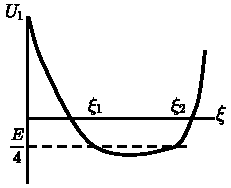
\includegraphics[width=4.2cm]{fig25.pdf}\\[0.3em]{\small 图 25}\end{minipage}\hfill
\begin{minipage}{0.48\linewidth}\centering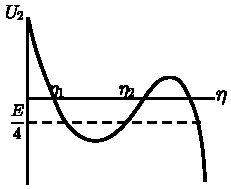
\includegraphics[width=4.2cm]{fig26.pdf}\\[0.3em]{\small 图 26}\end{minipage}
\end{minipage}\par\nopagebreak

\begin{equation}
\left.\begin{aligned}
  &\int_{\xi_1}^{\xi_2}\sqrt{2\left[\frac{E}{4}-U_1(\xi)\right]}\,\mathrm{d}\xi
  =\left(n_1+\frac{1}{2}\right)\pi,\\
  &\int_{\eta_1}^{\eta_2}\sqrt{2\left[\frac{E}{4}-U_2(\eta)\right]}\,\mathrm{d}\eta
  =\left(n_2+\frac{1}{2}\right)\pi.
\end{aligned}\right\}
\end{equation}
式中的 $n_1$ 和 $n_2$ 都是整数\footnote{详细的研究表明，把 $U_1$ 和 $U_2$ 中的 $m^{2}-1$ 改成 $m^{2}$ 后，可得更精确的结果.这样一来，整数 $n_1$ 和 $n_2$ 就等于抛物量子数.}.这两个式子隐含地确定了参量 $\beta_1,\beta_2$ 和 $E$ 的关系.再加上关系式 $\beta_1+\beta_2=1$，就能给出电场中移动能级的能量值.(77.13)式中的积分可以化成一些椭圆积分；这些方程式只能用数值方法求解.

强电场中的斯塔克效应由于另一现象而复杂化，这就是原子在外电场中的电离现象\footnote{C.~Lanczos, 1931.}.电子在外场中的势能 $\mathcal{E}z$，当 $z\rightarrow-\infty$ 时，可取任意大的负值.该电子在原子内的势能加上 $\mathcal{E}z$ 以后，结果使电子的运动区域增大（该电子的总能量 $E$ 是负的），除了原子的内部区域以外，还包括沿阳极方向的远离原子核的区域.这两个区域被一个势垒所隔开，势垒的宽度随着 $\mathcal{E}$ 的增大而递减.然而在量子力学中，粒子穿透势垒的概率并不等于零.在目前情形下，电子穿过势垒从原子内部逸出的现象，就是该原子的电离过程.弱电场中的这种电离概率小得几乎等于零.但是这个概率将随 $\mathcal{E}$ 的增大而指数式地增大，在足够强的电场中就不可忽视\footnote{这一现象提供了一个例证，说明小的微扰为什么有可能改变能谱的性质.即使是一个弱的电场 $\mathcal{E}$，也足以产生一个势垒和一个远离原子核的电子经典运动区.严格讲来，其结果是使电子的运动成为无限运动，从而使能谱由离散变成连续.但是，用微扰论方法求得的形式解仍有它的物理意义：这样给出的能级是属于这样的一些态，这些态虽然不完全是定态，但“差不多”都是定态.处于这样的一个态中的原子，将在很长时间内维持在这个态中.

可是，用微扰论计算能级的斯塔克分裂时，所得的级数并不是严格收敛的，它只是一个渐近级数：从该级数的某一项开始（微扰愈小，此项出现得愈晚），其后的项不是减小而是增大.}.

\begin{xiti}

\noindent{\heiti 习题1}\quad 试求氢原子（基态）在 $\mathcal{E}\ll1$（在通常单位制中为 $\mathcal{E}\ll m^{2}|e|^{5}/\hbar^{4}$）的电场中（每单位时间）的电离概率\footnote{本题采用原子单位.}.

解：在抛物坐标中“沿 $\eta$ 坐标轴”有一个势垒（图26）；电子沿 $z\rightarrow-\infty$ 方向从原子中被“拉出”，相当于它进入了 $\eta$ 值很大的区域.为了求出电离概率，必须研究 $\eta$ 值很大时（以及 $\xi$ 值很小时）波函数的形式（下面将看到，在求逸出电子总概率流量的积分式时，小的 $\xi$ 值是重要的）.基态电子的波函数（无外场时）为
\setcounter{equation}{0}\renewcommand{\theequation}{\arabic{equation}}%
\begin{equation}
  \psi=\mathrm{e}^{-\frac{1}{2}(\xi+\eta)}/\sqrt{\pi},
\end{equation}
当有外场存在时，在我们感兴趣的区域内 $\psi$ 和 $\xi$ 的关系可以看作和(1)式相同，至于它和 $\eta$ 的关系由下列方程确定：
\begin{equation}
  \frac{\partial^{2}\chi}{\partial\eta^{2}}
  +\left[-\frac{1}{4}+\frac{1}{2\eta}+\frac{1}{4\eta^{2}}+\frac{1}{4}\,\mathcal{E}\eta\right]\chi=0
\end{equation}
［即 $E=-\dfrac{1}{2}$，$m=0$，$\beta_2=\dfrac{1}{2}$ 的(77.11)第二式］，其中 $\chi=\sqrt{\eta}\,\psi$.令 $\eta_0$ 为 $\eta$ 的某个值（在势垒内），满足 $1\ll\eta_0\ll1/\mathcal{E}$.当 $\eta\geqslant\eta_0$ 时，波函数是准经典的.另一方面，由于(2)式呈一维薛定谔方程的形式，我们可以应用(50.2)式.作为边界条件，$\psi$ 在 $\eta=\eta_0$ 处应该变成(1)式的波函数，我们就得到势垒之外的下列表式：
\begin{equation*}
  \chi=\left(\frac{\eta_0|p_0|}{\pi p}\right)^{\frac{1}{2}}
  \exp\left(-\frac{\xi+\eta_0}{2}
  +\mathrm{i}\int_{\eta_0}^{\eta}p\,\mathrm{d}\eta+\frac{1}{4}\mathrm{i}\pi\right),
\end{equation*}
其中
\begin{equation*}
  p(\eta)=\sqrt{-\frac{1}{4}+\frac{1}{2\eta}+\frac{1}{4\eta^{2}}+\frac{\mathcal{E}\eta}{4}}.
\end{equation*}
我们只对平方 $|\chi|^{2}$ 感兴趣，因此指数幂的虚部并不重要.令 $\eta_1$ 为方程 $p(\eta)=0$ 的根，我们有
\begin{equation}
  |\chi|^{2}=\frac{\eta_0|p_0|}{\pi p}
  \exp\left(-\xi-2\int_{\eta_0}^{\eta_1}|p|\,\mathrm{d}\eta-\eta_0\right).
\end{equation}
$\eta\gg1$ 时，我们在上式指数前的系数中令
\begin{equation*}
  |p_0|\approx\frac{1}{2},
  \qquad
  p\approx\frac{1}{2}\sqrt{\mathcal{E}\eta-1}.
\end{equation*}
指数幂中必须保留 $p(\eta)$ 展式的下一项：
\begin{equation*}
  |\chi|^{2}=\frac{\eta_0}{\pi\sqrt{\mathcal{E}\eta-1}}
  \exp\left[-\xi-\int_{\eta_0}^{\eta_1}\sqrt{1-\mathcal{E}\eta}\,\mathrm{d}\eta
  +\int_{\eta_0}^{\eta_1}\frac{\mathrm{d}\eta}{\eta\sqrt{1-\mathcal{E}\eta}}-\eta_0\right],
\end{equation*}
其中 $\eta_1\approx1/\mathcal{E}$，积分后（$\eta_0\mathcal{E}$ 与1相比可略去）可得
\begin{equation}
  |\chi|^{2}=\frac{4}{\pi\mathcal{E}\sqrt{\mathcal{E}\eta-1}}
  \exp\left(-\xi-\frac{2}{3\mathcal{E}}\right).
\end{equation}
通过垂直于 $z$ 轴的一个平面的总概率流量（即欲求的电离概率 $w$）为
\begin{equation*}
  w=\int_0^{\infty}|\psi|^{2}v_z\,2\pi\rho\,\mathrm{d}\rho,
\end{equation*}
$\rho$ 为该平面内的圆柱半径.对于大的 $\eta$（以及小的 $\xi$）我们可令
\begin{equation*}
  \mathrm{d}\rho=\mathrm{d}\sqrt{\xi\eta}\approx\frac{1}{2}\sqrt{\frac{\eta}{\xi}}\,\mathrm{d}\xi
\end{equation*}
并把下列电子速度代入，
\begin{equation*}
  v_z\approx\sqrt{2\left(-\frac{1}{2}+\frac{1}{2}\mathcal{E}\eta\right)}
  =\sqrt{\mathcal{E}\eta-1},
\end{equation*}
我们有
\begin{equation*}
  w=\int_0^{\infty}|\chi|^{2}\pi\sqrt{\mathcal{E}\eta-1}\,\mathrm{d}\xi,
\end{equation*}
故最后得
\begin{equation}
  w=\frac{4}{\mathcal{E}}\exp\left(-\frac{2}{3\mathcal{E}}\right)
\end{equation}
用通常的单位制时，则得
\begin{equation*}
  w=\frac{4m^{3}|e|^{9}}{\mathcal{E}\hbar^{7}}
  \exp\left(-\frac{2m^{2}|e|^{5}}{3\mathcal{E}\hbar^{4}}\right).
\end{equation*}

\noindent{\heiti 习题2}\quad 求短程力势阱中的一个束缚 s 态电子被电场拉出的概率.假定电场很弱，满足 $|e|\mathcal{E}\ll\hbar^{2}\kappa^{3}/m$，其中 $\kappa=\sqrt{2m|E|}/\hbar$，$E$ 为阱中电子的结合能，$m$ 为电子质量\footnote{Ю.\,Н.\,Демков, Г.\,Ф.\,Друкарев, 1964}.

解：和例题1一样，对于弱电场，重要的是远距离（$\kappa r\gg1$）的情况.阱中电子的束缚态波函数（无电场）在该处具有渐近式
\begin{equation*}
  \psi=\frac{A\sqrt{\kappa}}{r}\,\mathrm{e}^{-\kappa r},
\end{equation*}
式中 $A$ 是一个与势阱形状有关的无量纲常数\footnote{例如，当势阱半径 $a$ 很小，以致满足 $a\kappa\ll1$ 时，则有 $A=1/\sqrt{2\pi}$；见 §133.}，用抛物坐标时，
\begin{equation*}
  r=\frac{1}{2}\left(\xi+\eta\right),
\end{equation*}
在 $\eta\gg\xi$ 区内波函数具有下列形式：
\begin{equation}
  \psi\approx\frac{2A\sqrt{\kappa}}{\eta}
  \exp\left[-\frac{1}{2}\kappa(\xi+\eta)\right],
\end{equation}
下面求解时质量、长度和时间的单位分别取 $m$，$\dfrac{1}{\kappa}$ 和 $\dfrac{m}{\hbar\kappa^{2}}$.

(6)式是 $\xi$ 函数和 $\eta$ 函数的乘积.当有电场存在时，$\psi$ 和 $\xi$ 的关系可以取作与(6)式相同（参见例题1）.为了求出 $\psi$ 和 $\eta$ 的关系，我们采用抛物坐标中的薛定谔方程.与库仑场情形不一样，势阱之场衰减很快，因此对本题至为重要的远距离处此场可以忽略.于是薛定谔方程分离变量后又得(77.11)式，在该式中现在必须令 $E=-\dfrac{1}{2}$ 和 $m=0$，且其分离参量现在满足条件
\begin{equation*}
  \beta_1+\beta_2=0.
\end{equation*}
参量 $\beta_1$ 应取 $\dfrac{1}{2}$［使得当 $\xi\mathcal{E}$ 很小时 $\psi\sim\mathrm{e}^{-\xi/2}$ 能够大致满足(77.11)式的第一个方程］；从而 $\beta_2=-\dfrac{1}{2}$，$\psi$ 是 $\eta$ 的函数，满足下列方程：
\begin{equation*}
  \frac{\partial^{2}\chi}{\partial\eta^{2}}
  +\left(-\frac{1}{4}-\frac{1}{2\eta}+\frac{1}{4\eta^{2}}+\frac{1}{4}\,\mathcal{E}\eta\right)\chi=0,
  \qquad \chi=\psi\sqrt{\eta}.
\end{equation*}
和(2)式一样解此方程，(3)式改成
\begin{equation*}
  |\chi|^{2}=\frac{4A^{2}|p_0|}{\eta_0 p}
  \exp\left(-\xi-2\int_{\eta_0}^{\eta_1}|p|\,\mathrm{d}\eta-\eta_0\right).
\end{equation*}
其中
\begin{equation*}
  p(\eta)=\sqrt{-\frac{1}{4}-\frac{1}{2\eta}+\frac{1}{4\eta^{2}}+\frac{\mathcal{E}\eta}{4}}.
\end{equation*}
其次，(4)式改成
\begin{equation*}
  |\chi|^{2}=\frac{A^{2}\mathcal{E}}{\sqrt{\mathcal{E}\eta-1}}
  \exp\left(-\xi-\frac{2}{3\mathcal{E}}\right),
\end{equation*}
最后，(5)式改成
\begin{equation*}
  w=\pi A^{2}\mathcal{E}\exp\left(-\frac{2}{3\mathcal{E}}\right),
\end{equation*}
用通常单位制时，得
\begin{equation*}
  w=\frac{\pi|e|\mathcal{E}A^{2}}{\hbar\kappa}
  \exp\left(-\frac{2\hbar^{2}\kappa^{3}}{3m|e|\mathcal{E}}\right).
\end{equation*}

\noindent{\heiti 习题3}\quad 求势阱中的一个电子受均匀可变电场 $\mathcal{E}=\mathcal{E}_0\cos\omega t$ 作用后，脱出阱外的概率（求出指数式精度即可），假定电场的频率和振幅满足下列条件：
\begin{equation*}
  \hbar\omega\ll|E|,
  \qquad
  |e|\mathcal{E}_0\ll\hbar^{2}\kappa^{3}/m.
\end{equation*}
其中 $\kappa=\sqrt{2m|E|}/\hbar$，$|E|$ 为阱中电子的结合能（Л.\,В.\,Кельдыш，1964）\footnote{这可作为一个例子，说明带单位负电荷的一个离子被强光所电离的情况；这里的势阱是由电子和中性原子实相互作用而产生的，条件 $\hbar\omega\ll|E|$ 保证了电磁波的场可作经典处理.}.

解：按所述条件，脱出概率 $w$ 是一个指数式小量.为了仅仅算出它的指数幂（不要求算出指数因子前的系数），只需考虑沿外场方向（$z$ 轴方向）的一维运动就足够了.

为方便计，电场最好用一个矢势（不是标势）$A_z=A=-c\mathcal{E}_0\sin\omega t/\omega$ 来描写.则阱外区的电子哈密顿量为［见(111.3)式］
\begin{equation*}
  \hat{H}=\frac{1}{2m}\left(-\mathrm{i}\hbar\frac{\partial}{\partial z}
  +\frac{|e|\mathcal{E}_0}{\omega}\sin\omega t\right)^{2},
\end{equation*}
式中不含 $z$.采用下列无量纲的变量和参量：
\begin{equation*}
  \tau=\frac{\hbar\kappa^{2}}{2m}\,t,
  \qquad
  \eta=2\kappa z,
  \qquad
  \Omega=\frac{2m\omega}{\hbar\kappa^{2}}=\frac{\hbar\omega}{|E|},
  \qquad
  F=\frac{|e|m\mathcal{E}_0}{\hbar^{2}\kappa^{3}},
\end{equation*}
可把薛定谔方程写成下列形式：
\begin{equation*}
  \frac{1}{4}\,\mathrm{i}\,\frac{\partial\psi}{\partial\tau}
  =-\left(\frac{\partial}{\partial\eta}
  +\frac{\mathrm{i}F}{\Omega}\sin\Omega\tau\right)^{2}\psi,
\end{equation*}
其边界条件为，解 $\psi(\eta,\tau)$ 当 $\eta\rightarrow0$ 时应该等于未受扰的阱内电子波函数（具有能量 $E=-|E|$）
\begin{equation}
  \eta\rightarrow0\ \text{时，}\ \psi\rightarrow\mathrm{e}^{\mathrm{i}\tau}.
\end{equation}
由于问题是准经典的，我们令具有指数式精度的解 $\psi$ 呈 $\psi=\exp(\mathrm{i}S)$ 形式，$S(\eta,\tau)$ 是经典作用量.由于哈密顿量与坐标 $\eta$ 无关，沿经典轨道的广义动量 $p_\eta=p$ 是守恒量.故
\begin{equation}
  S=-\int_{\tau_0}^{\tau}H(p,\tau')\,\mathrm{d}\tau'+\eta p+A,
  \qquad
  H(p,\tau)=4\left(p+\frac{F}{\Omega}\sin\Omega\tau\right)^{2},
\end{equation}
式中 $A$ 和 $\tau_0$ 是常数.根据作为坐标函数的作用量的含义（见《力学》，§43），$p$ 必须取轨道在 $\tau$ 时刻位于 $\eta$ 点的值，亦即把 $p$ 作为 $\eta$ 和 $\tau$ 的函数由运动方程 $\partial S/\partial p=$ 常数确定：
\begin{equation}
  \eta=\int_{\tau_0}^{\tau}\frac{\partial H(p,\tau')}{\partial p}\,\mathrm{d}\tau',
\end{equation}
式中的常数选得使 $\tau=\tau_0$ 时 $\eta=0$.(8)式和(9)式给出了作用量，它是 $\tau_0$ 和 $A$ 这两个常数的函数.为了获得满足(7)式条件的解（与求出哈密顿–雅可比方程的通解一样；见《力学》，§47附注），我们必须把 $A$ 看作是 $\tau_0$ 的函数，而 $\tau_0$ 作为坐标和时间的函数，由下式定义：
\begin{equation}
  \frac{\partial S}{\partial\tau_0}=0,
\end{equation}
显然有 $A(\tau_0)=\tau_0$；故当 $\eta=0$，$\tau=\tau_0$ 时，我们有 $S=\tau_0$，亦即 $S=\tau$，这和条件(7)完全一致.此时(10)式变成
\begin{equation}
  H(p,\tau_0)+1=0,
\end{equation}
(9)式和(11)式一起确定了 $\tau_0(\eta,\tau)$ 和 $p(\eta,\tau)$ 函数，从而［把它们代入(8)式后］确定了波函数 $\psi(\eta,\tau)$.

所求概率 $w$ 与沿 $z$ 轴的流密度成正比.在经典通区内，它等于 $v_z|\psi|^{2}$.经典通区开始点的坐标值，等于 $\mathrm{Im}\,S$ 不再增长时的点.在该点处 $(\partial\,\mathrm{Im}\,S/\partial\eta)_\tau=0$，由于 $\partial S/\partial\eta=p$，得 $\mathrm{Im}\,p=0$；再根据(9)式和(11)式我们可得 $\mathrm{Re}\,p=0$.根据这一条件，我们可以求出 $\tau_0$ 值，把 $p=0$ 代入(11)式后，得
\begin{equation*}
  \frac{4F^{2}}{\Omega^{2}}\sin^{2}\Omega\tau_0=-1,
\end{equation*}
从而有
\begin{equation*}
  \Omega\tau_0=\mathrm{i}\,\mathrm{arsinh}\,\gamma,
  \qquad
  \gamma=\frac{\Omega}{2F}=\frac{\sqrt{2m|E|\omega}}{|e|\mathcal{E}_0}.
\end{equation*}
“时间” $\tau_0$ 为虚数这一点说明了这个过程是经典不可能的.

\begin{equation*}
  w\sim\exp\left\{-2\,\mathrm{Im}
  \left[\int_{\tau}^{\tau_0}\frac{4F^{2}}{\Omega^{2}}\sin^{2}\Omega\tau'\,\mathrm{d}\tau'
  +\tau_0\right]\right\},
\end{equation*}
式中的 $\tau$ 可取任意实数值；积分的虚部不受影响.上式积出后，得
\begin{equation}
  w\sim\exp\left\{-\frac{2|E|}{\hbar\omega}\,f(\gamma)\right\},
  \qquad
  f(\gamma)=\left(1+\frac{1}{2\gamma^{2}}\right)\mathrm{arsinh}\,\gamma
  -\frac{\sqrt{1+\gamma^{2}}}{2\gamma},
\end{equation}
$f(\gamma)$ 函数的极限式为
\begin{equation*}
  f(\gamma)\approx\frac{2}{3}\gamma,
  \qquad(\gamma\ll1)
\end{equation*}
\begin{equation*}
  f(\gamma)\approx\ln 2\gamma-\frac{1}{2},
  \qquad(\gamma\gg1)
\end{equation*}
$\gamma\rightarrow0$ 时 $w$ 的极限值，相当于粒子被恒定场拉出阱外的概率.

(12)式只当指数幂很大时才能应用.为此，在任何情况下必须具有 $\hbar\omega\ll|E|$ 的条件.

\end{xiti}
\renewcommand{\theequation}{\arabic{section}.\arabic{equation}}%
